% !TEX TS-program = pdflatex
% !TEX encoding = UTF-8 Unicode

% This is a simple template for a LaTeX document using the "article" class.
% See "book", "report", "letter" for other types of document.

\documentclass[11pt]{article} % use larger type; default would be 10pt

\usepackage[utf8]{inputenc} % set input encoding (not needed with XeLaTeX)

%%% Examples of Article customizations
% These packages are optional, depending whether you want the features they provide.
% See the LaTeX Companion or other references for full information.

%%% PAGE DIMENSIONS
\usepackage{geometry} % to change the page dimensions
\geometry{a4paper} % or letterpaper (US) or a5paper or....
\geometry{margin=2in} % for example, change the margins to 2 inches all round
% \geometry{landscape} % set up the page for landscape
%   read geometry.pdf for detailed page layout information

\usepackage{graphicx} % support the \includegraphics command and options
\usepackage{fullpage}

% \usepackage[parfill]{parskip} % Activate to begin paragraphs with an empty line rather than an indent

%%% PACKAGES
\usepackage{booktabs} % for much better looking tables
\usepackage{array} % for better arrays (eg matrices) in maths
\usepackage{paralist} % very flexible & customisable lists (eg. enumerate/itemize, etc.)
\usepackage{verbatim} % adds environment for commenting out blocks of text & for better verbatim
\usepackage{subfig} % make it possible to include more than one captioned figure/table in a single float
% These packages are all incorporated in the memoir class to one degree or another...

%%% HEADERS & FOOTERS
\usepackage{fancyhdr} % This should be set AFTER setting up the page geometry
\pagestyle{fancy} % options: empty , plain , fancy
\renewcommand{\headrulewidth}{0.5pt} % customise the layout...
\lhead{}\chead{Smart Refrigerator Proposal}\rhead{}
\lfoot{}\cfoot{\thepage}\rfoot{}
\addtolength{\topskip}{+0.5cm}

%%% SECTION TITLE APPEARANCE
\usepackage{sectsty}
%\allsectionsfont{\sffamily\mdseries\upshape} % (See the fntguide.pdf for font help)
% (This matches ConTeXt defaults)

%%% ToC (table of contents) APPEARANCE
\usepackage[nottoc,notlof,notlot]{tocbibind} % Put the bibliography in the ToC
\usepackage[titles,subfigure]{tocloft} % Alter the style of the Table of Contents
%\renewcommand{\cftsecfont}{\rmfamily\mdseries\upshape}
%\renewcommand{\cftsecpagefont}{\rmfamily\mdseries\upshape} % No bold!

\usepackage{amsmath}
%\usepackage{amsfonts}
%\usepackage{amssymb}
\usepackage[normalem]{ulem}
\usepackage{url}
\usepackage{graphicx}

%1 Exercise number
%2 Exercise name
%3 Date performed
%4 Date submitted
\newcommand{\coversheet}[4]{
  \begin{titlepage}
    \setlength\topmargin{2in}
    \begin{center}
      \Huge\textsc{Smart Refrigerator Proposal}\\
      \vspace{.125in}
      \hrule
      \vspace{.125in}
      \normalsize
      \today \\
      \vspace{.375in}
      This project will develop a prototype “Smart Refrigerator” system, which will monitor grocery items purchased by the user in order to reduce food waste and facilitate efficient shopping habits. 

    \end{center}
    \vfill
    \hspace{4.2in} Steven Strapp - ses6498@rit.edu
    
    \noindent \hspace{4.2in} Computer Engineering Year 4

    \noindent \hspace{4.2in} 

    \noindent \hspace{4.2in} Ben Reeves - bpr5171@rit.edu
    
    \noindent \hspace{4.2in} Computer Engineering Year 5

    \noindent \hspace{4.2in} 

    \noindent \hspace{4.2in} Dustin Stroup - dxs2857@rit.edu

    \noindent \hspace{4.2in} Computer Engineering Year 5

    \quad \newline \newline \newline \newline \newline \newline \newline \newline
  \end{titlepage}
}

%1 label
%2 number of variables
%3 kmap label
%4 variables
%5 truth table
%6 Marks
%7 Prime implicants table
%8 Final EQ
\newcommand{\kmap}[8]{
  \begin{center}
    \begin{tabular}{l}
      \multicolumn{2}{c}{\underline{#1}} \\  
        \karnaughmap{#2}{#3}{#4}{#5}{
		#6        
        }
      #8
    \end{tabular}
  \end{center}
  }

%1 figure position
%2 figure scale
%3 path to photo
%4 Caption
%5 reference lable
\newcommand{\pic}[5]{
\begin{figure}[#1]
  \begin{center}
    \includegraphics[scale=#2]{#3}
    \caption{#4}
    \label{#5}
  \end{center}
\end{figure}
}



\begin{document}
\coversheet{V}{\textsc{Kinetis K60 Based Electrocardiogram}}{October 28, 2011}{November 11, 2011}
\setcounter{page}{2}

\addtolength{\topskip}{+0.5cm}
\tableofcontents
\addtolength{\topskip}{-0.5cm}
\pagebreak
\section{Overview}
\subsection{Needs Statement}
The New York Times reports that an average American family of four will account for over 120 pounds of food waste per month and that 27\% percent of all food available will be lost to waste \cite{times}. In addition, other resources are lost due to inefficient shopping practices; forgetting common items or special trips made for recipe ingredients waste time and fuel. A system is required for shoppers both to ensure their purchases are used before expiration and to assist in planning of grocery shopping trips.
\subsection{Objective Statement}
The objective of this project is to design a prototype that will allow a user to track food items in order to reduce waste and improve shopping efficiency. The system will remind the user about items nearing their expiration date and track the frequency of purchased items. From this frequency calculation the system will suggest typical shopping lists. A mobile phone application will provide an interface to the unit to view or create shopping lists and to query inventory.
\subsection{Description}
A UPC scanner will be used to identify items added or removed from the refrigerator's inventory; a database of UPC codes will translate from the scanned code to an item description. Two databases will be maintained, one linking UPC codes to product descriptions and expiration dates and another to store items currently checked into the refrigerator. A central processing platform on the base station will be used to decode UPC information and to store and interact with the databases. This platform will provide a web interface accessible both via a display on the main unit and also using a mobile interface. The display on the main unit will allow a user both to check current inventory with expiration dates and to provide additional information when adding or removing items. Both the base station and mobile interfaces can also be used to display and modify suggested shopping lists. The mobile application will interact with the same web interface but will provide a graphical interface optimized for smaller displays. The system will continually estimate the frequency that particular items are purchased and will use this information, combined with the expiration dates and purchase dates, to suggest shopping lists. In addition to shelf life, temperature is also a critical factor for food storage systems. To address this need the system will incorporate a temperature and humidity sensor, and this information will be accessible through the mobile application.
\newline \quad \newline
A high level system diagram isolating components is shown in Figure \ref{fig:sysdiag}.
\begin{figure}[h]
\begin{center}
\vspace{0.5cm}
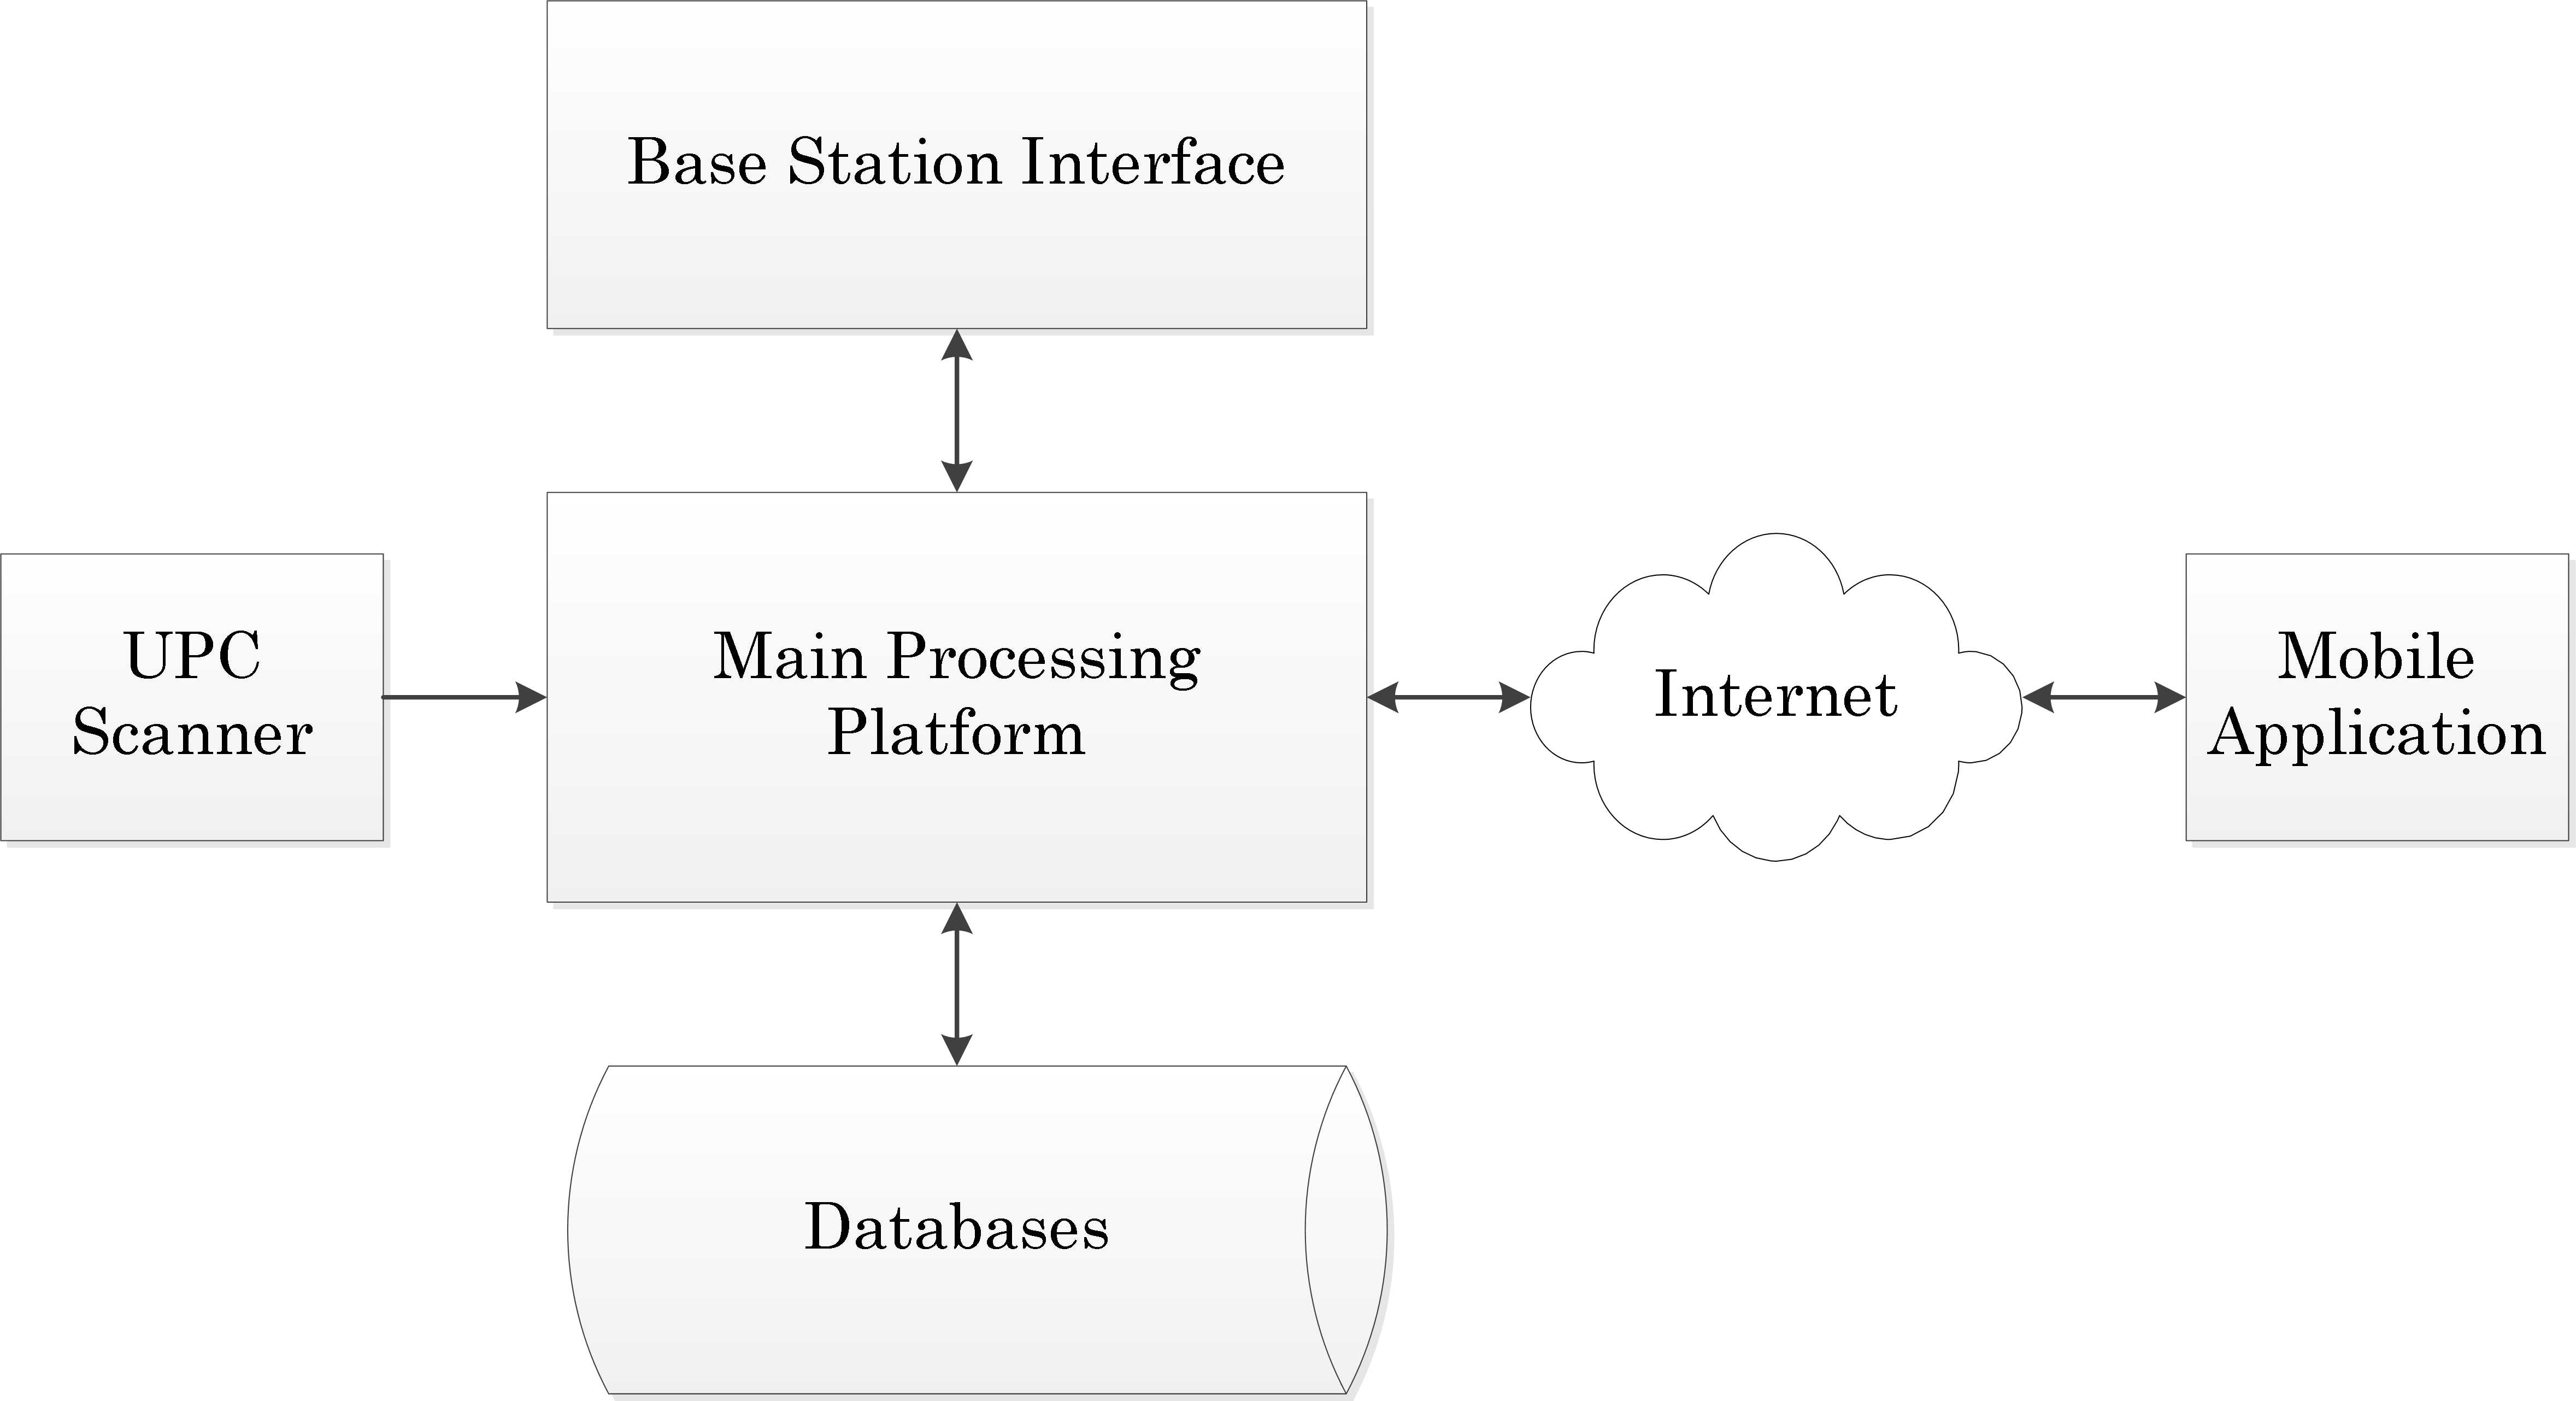
\includegraphics[scale=0.7]{HighestLevelDiagram}
\caption{High Level System Diagram}
\label{fig:sysdiag}
\end{center}
\end{figure}
\pagebreak
\section{Requirements Specification}
\subsection{Customer Needs}
\begin{enumerate}
\item The system should provide an intuitive, easy to use graphical interface.
\item The system should require minimal user input.
\item The system should be able to scan product codes and identify corresponding items quickly.
\item The system should provide secure remote access.
\item The system should report items nearing expiration.
\item The system should provide access to the current inventory.
\item The system should provide a method to create and edit shopping lists.
\item The system should recommend shopping lists which accurately reflect buying habits.
\item The system should function as an add-on to an existing refrigerator or pantry.
\item The system should indicate if food products are stored safely.
\end{enumerate}
\pagebreak
\subsection{Engineering Specifications}
\begin{table}[h!]
\begin{center}
\begin{tabular}{| p{1.2in} | p{2.5in} |p{2.5in} |}
\hline
Customer Need & Engineering Requirement & Justification \\
\hline
2,3 &A. An off-the-shelf UPC scanner should be used to input items. & A UPC scanner can read product codes with a single click.\\
\hline
3 &B. An internal UPC code database should be used to associate codes with items.&An internal database will remove delays associated with an internet look-up.\\
\hline
1,4,6&C. The system should be internet enabled and provide a web interface.&By providing a web interface any other internet-connected device can access the system.\\
\hline
4&D. Remote access should be authenticated with user name and password.&User names and passwords are standard for access control.\\
\hline
2,5&E. An internal database will store default recommended expiration estimates for common categories of items.&Inferring expiration dates based on item category helps minimizes user input. It is well known how long some products take to expire.\\
\hline
1,5&F. The user interface will provide a method for updating default expiration estimates.&Default estimates will not account for condition of product on arrival and may need to be updated.\\
\hline
1,5&G. Interface will provide a visual indication to the user when items are within a user-defined margin of expiration.&The goal of the system is to reduce waste due to expiration.\\
\hline
1,6&H. From both the base station and mobile application the user will be able to view an inventory list.&The user needs access to the current inventory in order to use items and shop effectively.\\
\hline
7,8&I. A database will be devoted to storing recommend shopping lists produced by the system.&User may wish to retain generic shopping lists for future use.\\
\hline
8&J. Recommended shopping lists will reflect purchasing history and expiration dates of current inventory.&Recommendation policy must suggest items relevant to the user in order to be useful.\\
\hline
7&K. Custom shopping lists, created either from the base station or the mobile interface, can be added to shopping list database.&Inefficient shopping practices can be prevented by storing shopping lists and the system can not anticipate all required items.\\
\hline
9&L. The system will be self-contained and no modifications will be required to existing appliances.&Similar systems are commercially available but require costly replacement of existing appliances.\\
\hline
10&M. The system should measure temperature and humidity within the refrigerator. & Temperature and humidity measurements will allow the user to determine if food storage conditions are safe. \\
\hline
\end{tabular}
\end{center}
\end{table}
\pagebreak
\section{Concept Selection}
\subsection{Evaluation of Existing Systems}
Many refrigerator systems are current available which offer integrated displays and internet connectivity. LG, Electrolux, and Samsung all offer refrigerators with large LCD displays that provide access to calendar applications, recipes, weather forecasts, and music and photo sharing services. The principle shortcoming of these devices is the elevated price and the need to completely replace existing appliances. As a more affordable alternative, tablet mounts are available for refrigerators as well.
However, these systems do not offer tracking of the refrigerator's contents and do not attempt to reduce waste or improve efficiency. In April of 2011, LG demonstrated a ``Smart Fridge" with goals closer to the proposed system. The sensors and algorithms used were not disclosed but the product objective is similar, tracking user purchases and providing a mobile interface to the refrigerator's contents while shopping \cite{lg}. Our system will provide a much more inexpensive alternative and will be more flexible; the system proposed will not be strictly limited to refrigerators and can be used as an add-on to an existing system.
\newline \quad \newline
Many patents exist on inventions related to the smart refrigerator system as a whole and its goal to reduce waste, but do not attempt to reduce user input. Patents 2004/0085225 A1 \emph{Methods and Apparatus to Monitor the Inventory of a Food Storage Unit}, 2010/0148958 A1 \emph{Expiration Warning Device of Refrigerator}, and 2011/0109453 A1 \emph{Apparatus for Warning of an Expiration Date} all treat the goals of the overall system but rely on the user to enter expiration dates manually. More advanced systems, as in Patents 7,861,542 B2 \emph{Refrigerator Including Food Product Management System} and 2011/016555 A1 \emph {Refrigerator and Control Method Thereof}, use radio frequency identification (RFID) tags attached to foods to read expiration dates, with user input as a fallback. The prototype designed will improve the simple user-intensive method of the first group but without the added scope of radio frequency identification used in the second group.
\subsection{Concepts Considered and Chosen}
Many of the system design choices are easily derived from the engineering requirements; a UPC scanner with a standard USB interface is a clear choice for input of product codes and a mobile application is an obvious interface choice for a system catering to an on-the-go shopper. However, the choices of implementation platform and main base station display present more alternatives. Expiration date recognition is also a potential shortcoming of the system; ideally image processing could be employed to read expiration dates. However, the difficulty and computational complexity of applying image processing significantly extends the scope of the project and places additional performance constraints on the processing platform used. An evaluation of different expiration date recognition systems is tabulated in Table \ref{tab:datesys}. The different evaluation criteria, ease of use, feasibility and accuracy, are at odds and each criteria was given equal weight during concept selection.
\begin{table}[h!]
\vspace{0.5cm}
\caption{Comparison of Expiration Date Systems}
\begin{tabular}{| p{1in} | p{1.15in} | p{1.15in} | p{1.15in} | p{1.15in}  | p{1.15in} |}
\cline{2-5}
\multicolumn{1}{c}{}&\multicolumn{4}{|c|}{Method} \\
\cline{2-5}
\multicolumn{1}{c|}{}&User Input \newline of expiration \newline dates& Image to Text \newline Recognition & Predictive \newline Strategy without \newline itemMaster& Predictive \newline Strategy with \newline itemMaster \\
\hline
Ease of Use&- - -&+&+ + +&+ + +\\
\hline
Feasibility&+ + +&- - -&- - -&+ + +\\
\hline
Accuracy & + + & + + &+&+\\
\hline \hline
Total &2+ &0&4+&7+\\
\hline
\end{tabular}
\label{tab:datesys}
\end{table}
\newline \quad \newline
Ease of use is one of the most critical system requirements; a system relying completely on input from the user will not be acceptable to consumers. However, feasibility and limiting processing performance required are important secondary objectives. Accuracy is critical to the goal of reducing waste due to expiration, but there is inherently some variability even in reported expiration dates. Image processing presents too much additional scope and too many additional requirements in exchange for marginal gains. As long as the predictive system learns from user input and anticipates that items will be purchased in different conditions, this scheme should be sufficient. One additional risk posed by the predictive system, the problem of deciphering text descriptions in order to assign an appropriate prediction, has been mitigated by using the ItemMaster UPC database. Many websites, such as the Food and Drug Administration or community based resources like \url{www.stilltasty.com}, provide ``rule of thumb" style predictions for expiration dates. However, the system must associate a product description with a rule of thumb which, after investigation, appears to be a difficult classification problem. The ItemMaster UPC database provides not only an association between a UPC code and a text description but also provides a GS1 category. There are a modest number of GS1 categories applicable to this system, each of which can be assigned a rule of thumb to initialize the prediction system.
\newline \quad \newline
The problem of predicting shopping habits will be formulated as a problem of predicting the probability that the user will purchase a product again after N days from the last purchase. A product will be added to the shopping suggestions at the peaks in the probability density function, after which the process would reset. To evaluate modeling strategies, receipts were retrieved for a three month interval from a single user. An initial attempt was to assume that the large number of factors influencing shopping habits could be approximated as normally distributed. However, for the data tested, this approximation was very poor; the data considered were either multi-modal or contained a single mode with outliers. In all cases considered, the distribution was shifted to the point where the most likely suggestion time was actually positioned in an interval not supported by any of the samples. A more advanced approach, a non-parametric distribution estimate, was considered next; this method outperformed the simple normal approximation, but appeared to interpolate more than necessary and was the most computationally complex method considered. A final approach clustered the data points, approximated each cluster with a normal distribution, and summed these distributions. With this strategy, each mode can be captured without the influence of outliers. The accuracy of the methods considered were evaluated both qualitatively, by looking at the resulting probability density functions, and also quantitatively, by considering performance on the example sets. Overall, clustering to produce a sum of Gaussians appears to be the optimal prediction strategy and the probability metrics used are tabulated in Table \ref{tab:pugh2}. The two goals of this subsystem, maximizing the probability of accurate recommendations and minimizing the probability of unsupported recommendations, were given equal weight during concept selection.

\pagebreak
\begin{table}[h!]
\vspace{0.5cm}
\caption{Comparison of Distribution Estimate Performance Metrics}
\begin{tabular}{| p{1.25in} | p{.25in} | p{1.25in} | p{1.25in} | p{1.25in} |}
\cline{3-5}
\multicolumn{2}{c}{}&\multicolumn{3}{|c|}{Method} \\
\cline{2-5}
\multicolumn{1}{c|}{}&\multicolumn{1}{|c|}{Trial}&Normal \newline Approximation&Non-Parametric \newline Distribution&Clustering to\newline produce sum of\newline Gaussians\\
\hline
\multicolumn{1}{|c|}{$\sum$ Log Probability} &1&-38.3394&-35.9682&-34.7721 \\
\cline{2-5}
\multicolumn{1}{|c|}{Observed Habits} &2&-20.5647&-17.0897&-15.6641 \\
\cline{2-5}
\multicolumn{1}{|c|}{(Goal to Maximize)} &3&-47.8101&-44.9658&-43.9845 \\
\cline{2-5}
\multicolumn{1}{|c|}{} &4&-29.1931&-19.6762&-24.4915 \\
\hline
\multicolumn{1}{|c}{Evaluation}&&- - -&-&+ + +\\
\hline
\multicolumn{1}{|c|}{$\sum$ Log Probability} &1&-36.7898&-38.4187&-50.6578\\
\cline{2-5}
\multicolumn{1}{|c|}{Habits Not} &2&-188.514&-225.002&-318.926 \\
\cline{2-5}
\multicolumn{1}{|c|}{Observed} &3&-62.2909&-63.8609&-69.9759 \\
\cline{2-5}
\multicolumn{1}{|c|}{(Goal to Minimize)} &4&-29.6667&-$\infty$&-86.0767 \\
\hline
\multicolumn{1}{|c}{Evaluation}&&- - -&+&+ +\\
\hline
\multicolumn{2}{|c|}{Ease of Computation} &+ + + &- - -&-\\
\hline \hline
\multicolumn{1}{|c}{Total}& &3- &3-&4+\\
\hline
\end{tabular}
\label{tab:pugh2}
\end{table}

\quad \newline
The choice of the base station main display and processing platform are linked but directed mainly by the processing platform. For example, if a personal computer were used a standard LCD monitor may be appropriate, whereas if a tablet were chosen as the main processing engine the interface would be provided automatically. The most strongly considered option was to use a simple micro-controller or BeagleBoard to handle the processing load and to use a large, relative to the micro-controller, LCD display. Comparisons of different processing platform methods and different user interface choices for the base station are shown in Tables \ref{tab:proc} and \ref{tab:disp}, respectively. The evaluation criteria for the processing platform and user interface were given equal weight; though since the processing platform and user interface concepts were related, the criteria of the processing platform were given higher priority than the user interface.
\begin{table}[h!]
\caption{Comparison of Main Processing Platforms}
\begin{tabular}{| p{1.5in} | p{.75in} | p{1.5in} | p{0.75in} | p{1.15in} | }
\cline{2-5}
\multicolumn{1}{c}{}&\multicolumn{4}{|c|}{Method} \\
\cline{2-5}
\multicolumn{1}{c|}{}&Personal \newline Computer&Tablet (Combined UI \newline and Processing)&Micro-controller & Beagleboard-xM\\
\hline
Processing Resources&+ + + +&+ +&+&+ + +\\
\hline
Cost &- - -& + &+ + +&+ + +\\
\hline
Size&- - -&+ +&+ + +& + + +\\
\hline
\hline
Total &2-&5+&7+& 9+\\
\hline
\end{tabular}
\label{tab:proc}
\end{table}

\begin{table}[h!]
\vspace{0.5cm}
\caption{Comparison of Main User Interface Displays}
\begin{tabular}{| p{2in} | p{1in} | p{1.5in} | p{1.5in} | p{1.5in} |}
\cline{2-4}
\multicolumn{1}{c}{}&\multicolumn{3}{|c|}{Method} \\
\cline{2-4}
\multicolumn{1}{c|}{}&LCD PC \newline Monitor&Tablet&LCD with \newline BeaglBoard-xM\\
\hline
Integration with Unit&- - -&-&+ + +\\
\hline
Ease of Use&+ + +&+ + +&+ +\\
\hline
Size of Display& + + + &+ + +&+ +\\
\hline
GUI Quality&+ + +&+ + +&+ + +\\
\hline
Size of Unit&- - -&+ + +&+ + +\\
\hline
\hline
Total&3+&12+&13+\\
\hline
\end{tabular}
\label{tab:disp}
\end{table}
\noindent Evaluating both the interface choice and the processing platform choice together eliminates the personal computer choice; a personal computer cannot be integrated without significantly increasing the form factor of the system. A personal computer also greatly simplifies the system and strays away from an implementation tailored to this prototype. A tablet based interface was considered a very feasible alternative; however the cost and tailorability of the system are again concerns. A micro-controller based system is more appropriate for a small and specialized solution, with the principle concern being quality of the graphical interface produced compared with the other two methods. However, since the system will provide a general web interface, the mobile application as well as a variety of other possible interfaces can be used to view the display as well. Thus, the weight assigned to a high-quality base station interface is mitigated. Considering both choices together, the Beagleboard-xM with an LCD display to inspect items visually as they are checked in and view inventory appears preferable.
\section{Design}
Consideration of the these concepts, as well as the high level system diagram presented in Figure \ref{fig:sysdiag}, clarifies the separation of tasks while implementing the project. One group of tasks will contain the mobile interface and also development of an Interface Control Document (ICD) to enumerate the commands provided over the web interface. A second task group will consist of configuring the internal databases on the Beagleboard, the expiration date warning system, and the shopping list suggestion algorithm. The final group of tasks will consist of interfacing the processing platform with the scanner, Ethernet interface, temprature and humidity sensor, and main user interface. The development of the base station interface will be distributed over the last two task groups. This division of work is also evident in the full system diagram shown in Figure \ref{fig:fullsys}.
\begin{figure}[h!]
\vspace{0.5cm}
\begin{center}
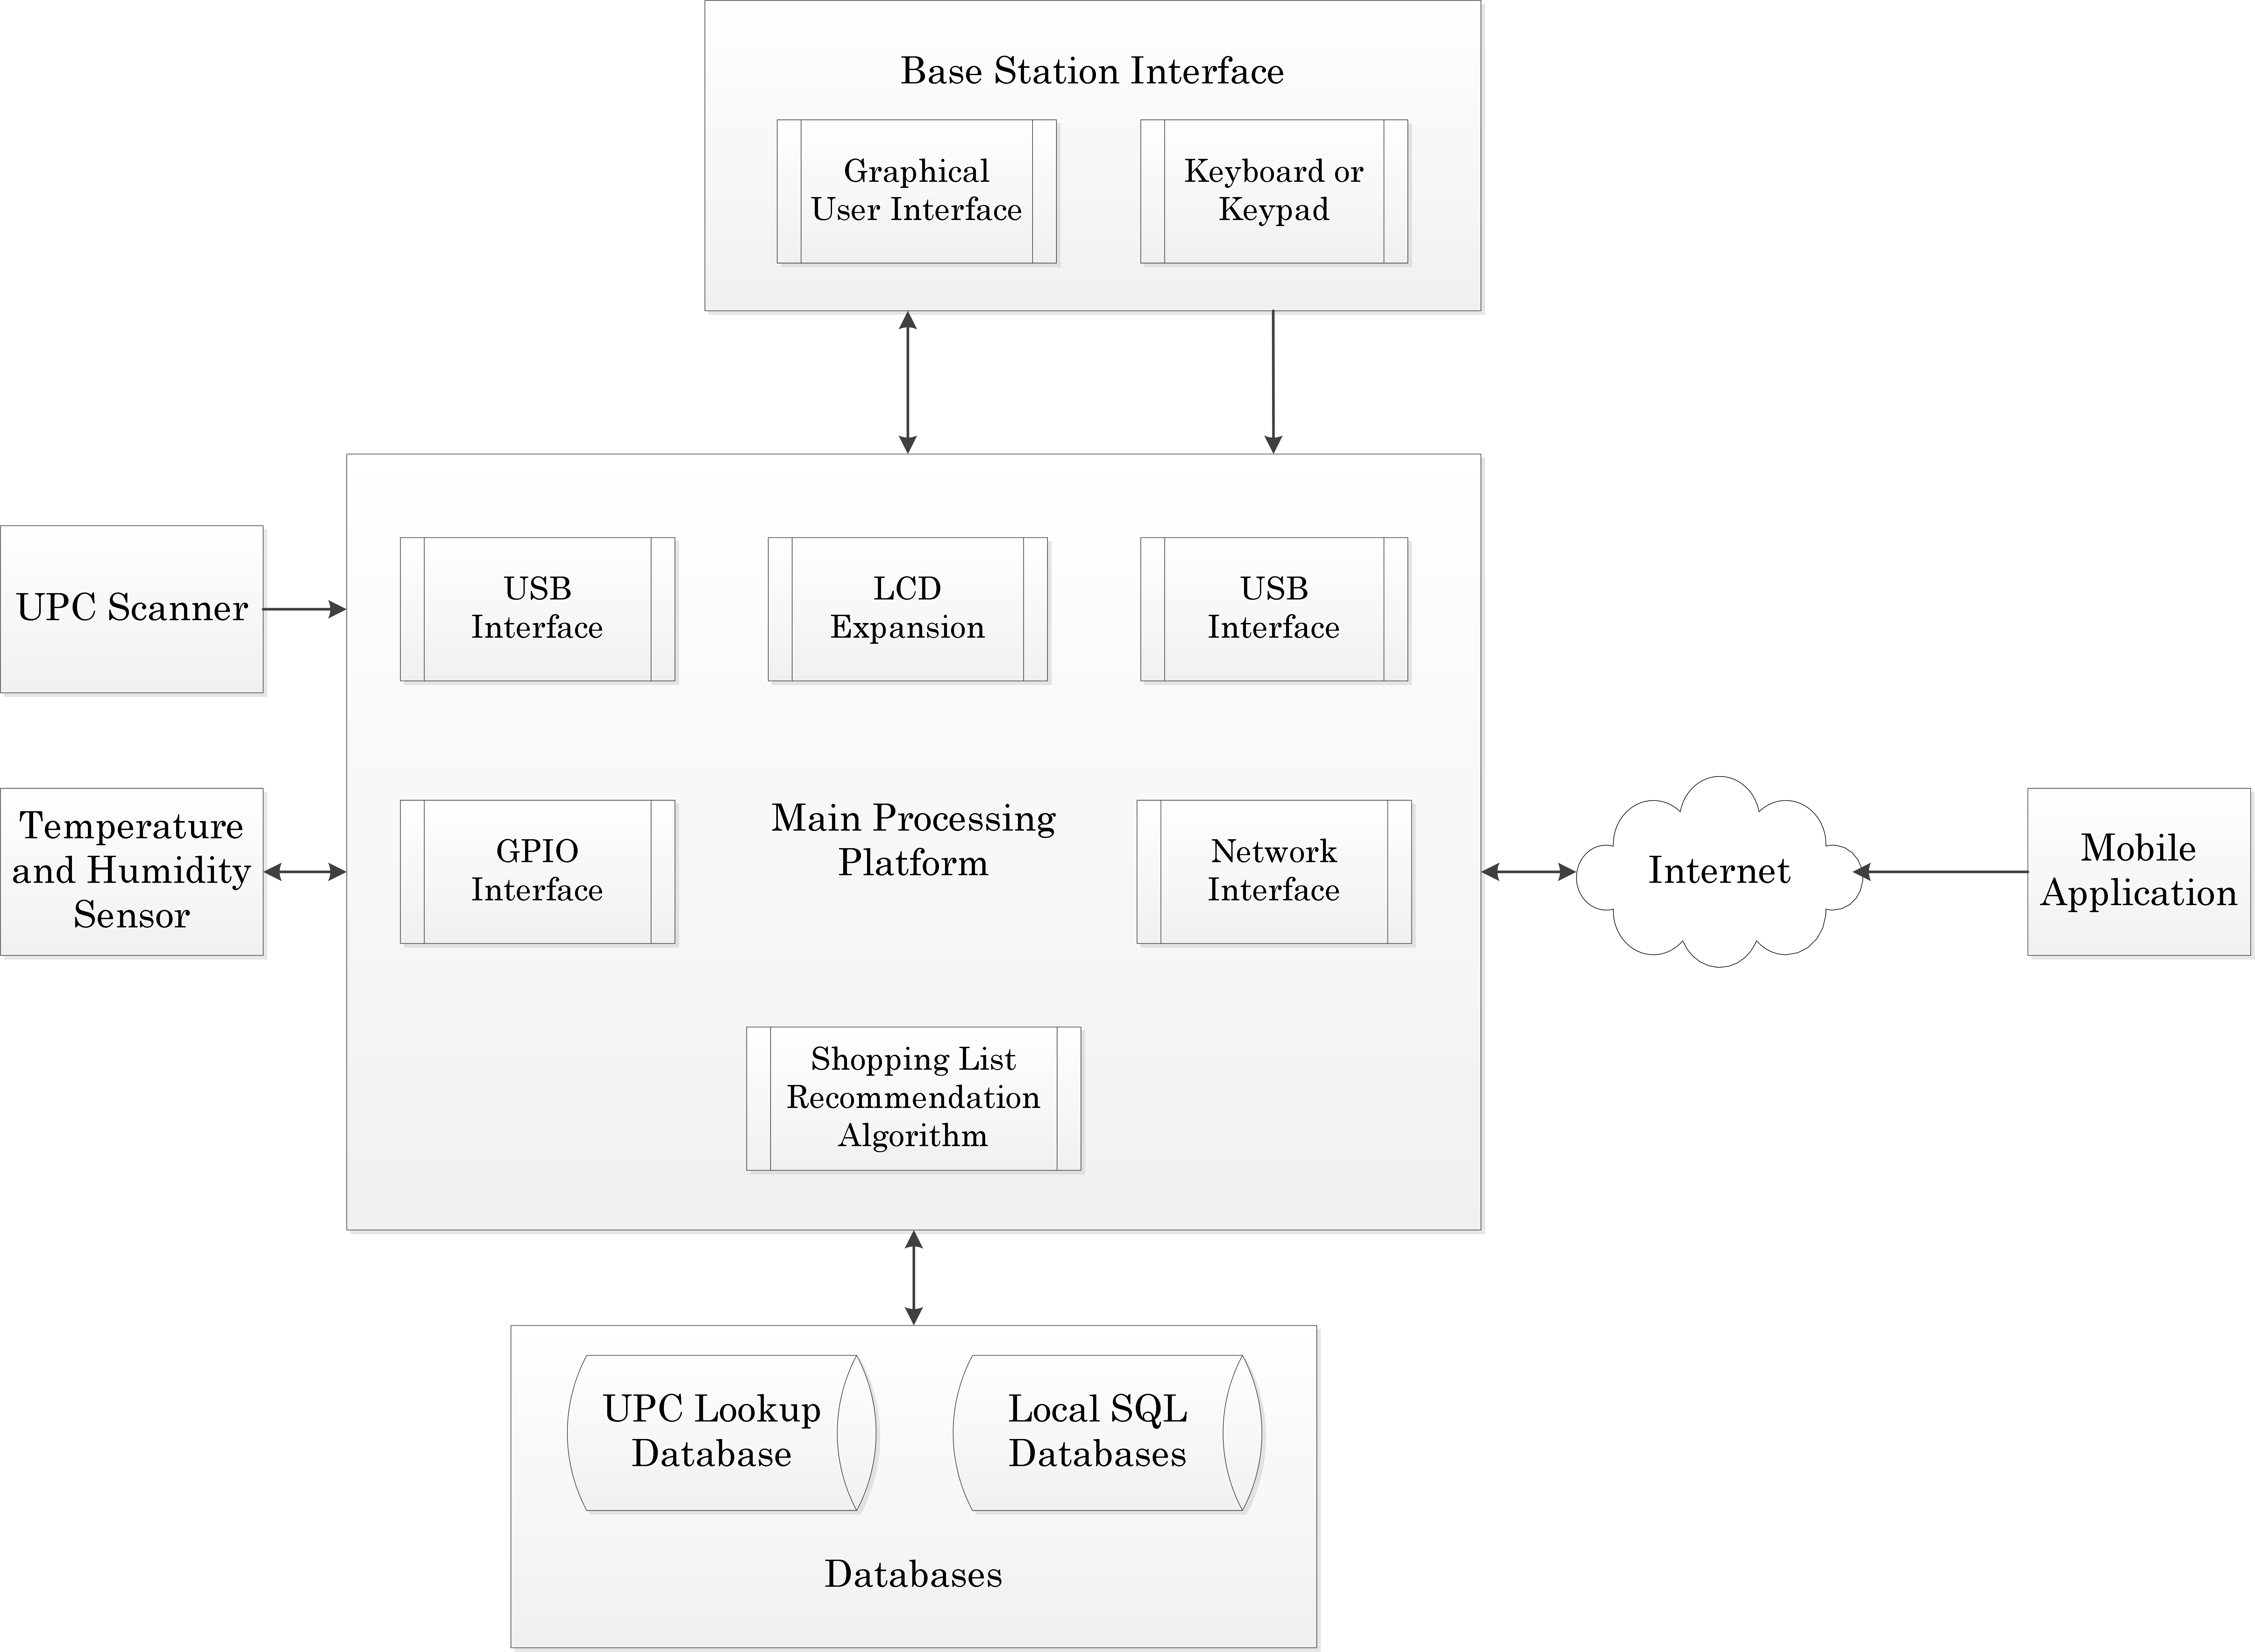
\includegraphics[scale=0.5]{../Graphics/FullSystemDiagram}
\caption{Full System Diagram}
\label{fig:fullsys}
\end{center}
\end{figure}
The majority of software developed will run on the Beagleboard, which will be the main processing platform for the Smart Refrigerator system. The Beagleboard will run the Angstrom operating system, a lightweight embedded Linux. A full Linux environment will be very conducive for software development and will greatly simplify connection with peripherals; the keypad or keyboard, as well as the UPC scanner, will be able to simply ``plug-and-play". The temperature and humidity sensor will require more effort, particularly to ensure the input and output voltage levels meet the specifications of the sensor and do not damage the Beagleboard. The RHT03 humidity and temperature sensor that will be used requires a 3.3V-6V power supply and will output voltages as high as the supply voltage. The Beagleboard's general purpose input and output (GPIO) pins supply and receive voltages up to 1.8V only; however, the pins also include a built-in level shifter. Since a level shifter is built in this constraint does not imply a need for extra circuitry; though care must be taken to configure the level shifter properly to avoid overvolting the GPIO inputs.
\newline \indent \newline
A more detailed diagram of the Beagleboard subsystem is shown in Figure \ref{fig:basecode}. The figure shows all external connections to the Beagleboard as well as an internal separation of sub-components. The base station code will be inspired by the Model, View, Controller paradigm. A distinct module of code will create the user interface displayed on the Beagleboard's touchpad and relay user interface events to a separate controller module. The controller sub-component will coordinate the various input events generate by the system. Input from the UPC scanner and keyboard will pass through this module and then be transferred to the view. The controller is a necessary middleman in this process, since scanned UPC codes and user inputs must be shared with the model as well. The controller will also be responsible for handling input from the temperature and humidity sensor; this interaction will occur through a dedicated GPIO driver. The controller must also interact with the database structures and handle event from the network interface. The model itself will be distributed among the remaining modules; the content needed by the model will be sorted within the databases, and the principle modeling task will occur within the expiration date and shopping list prediction sub-module. The two prediction algorithms will be separated as a unique subsystem, since the prediction task is a unique portion of the system and will belong to a different task group than the overall base station software application.
\begin{figure}[h!]
\vspace{0.5cm}
\begin{center}
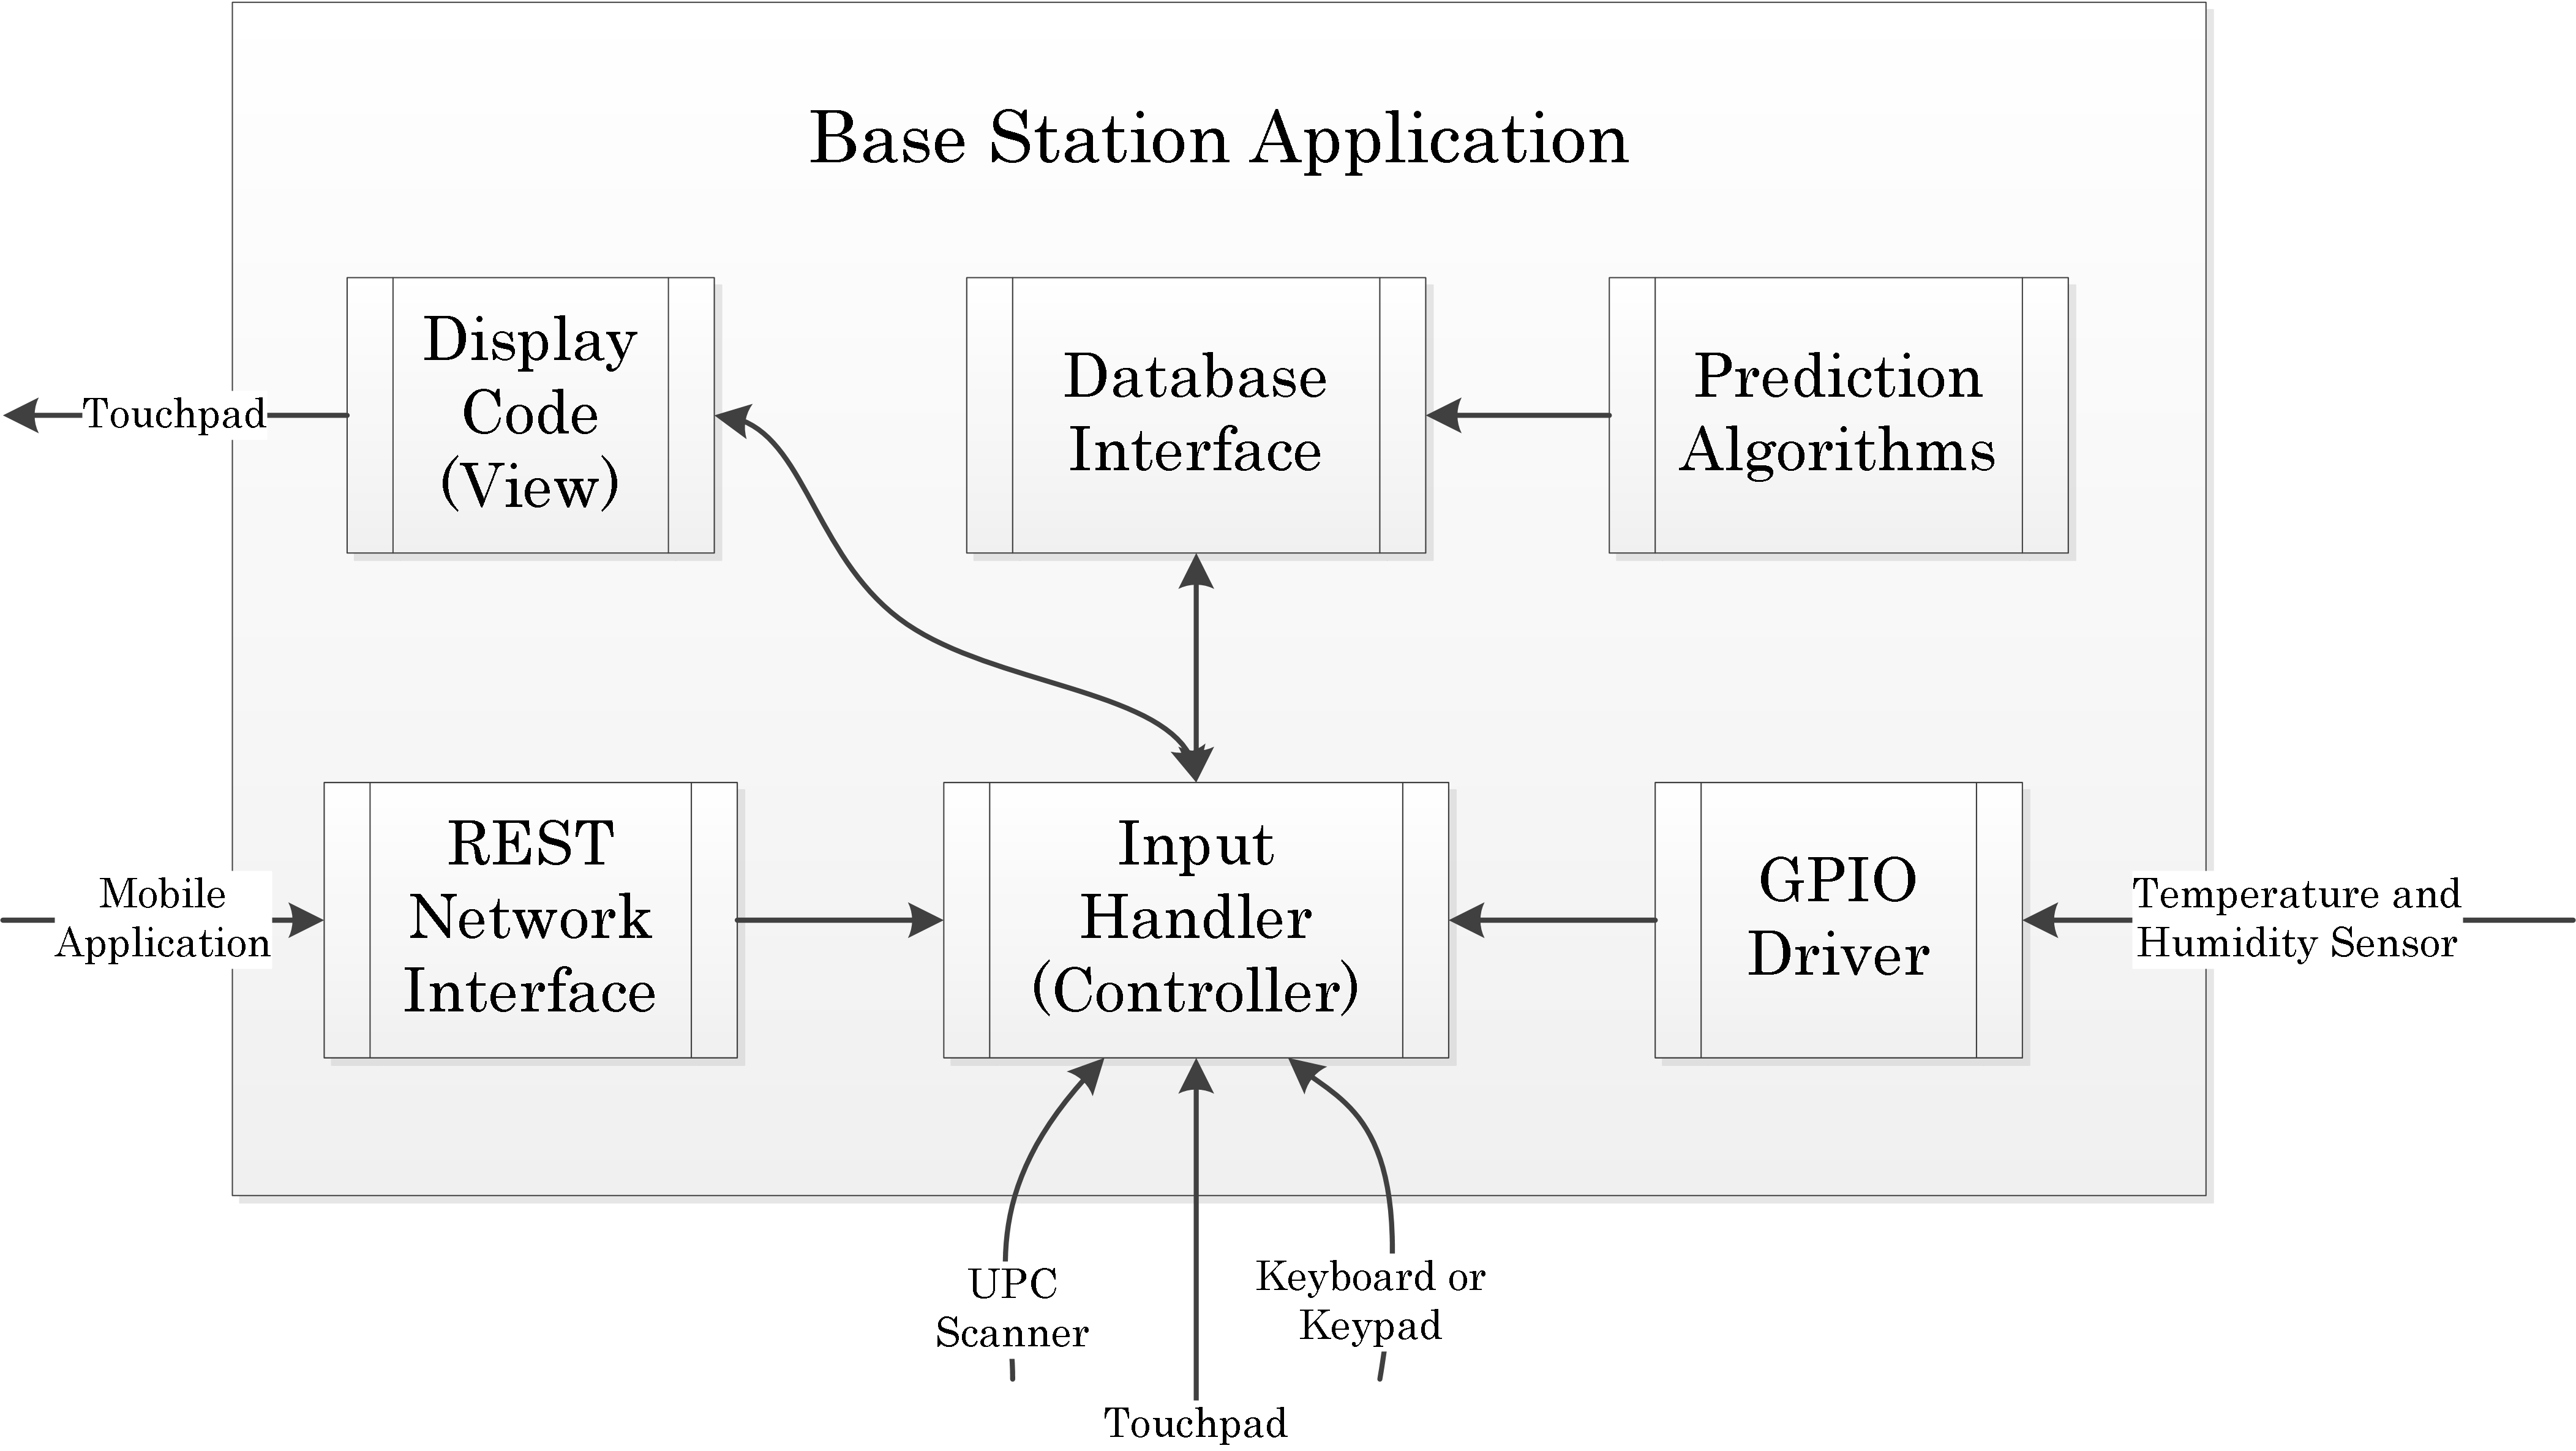
\includegraphics[scale=0.8]{../Graphics/BaseStation}
\caption{Beagleboard Subsystems}
\label{fig:basecode}
\end{center}
\end{figure}
\newline \quad \newline
The base station application will be developed in C++ using the Qt user interface framework. Java was also given consideration as the primary language, since this could potentially increase consistency with the mobile application. However, C++ appeared to be a much more common language across the existing drivers and code examples provided for the Beagleboard. Effort will still be made to maintain consistency between the two user interfaces. To facilitate ease of use and a fluid user experience between the two applications, the interface layout should be preserved exactly, and aesthetic differences should be minimized. Some initial layouts for the graphical user interface have been designed and are shown in Figures \ref{mock1}, \ref{mock2}, \ref{mock3}, and \ref{mock4}. When designing the interface layouts, the constraints of a touch screen interface were considered; all buttons and tabs are intentionally large and easy to click. The Product Entry tab will be the default, and will provide feedback to the user while scanning items. The ``Check In" and ``Check Out" buttons will function as radio buttons to indicate whether the next scanned item will be interpreted as a new purchase or an item being removed from the current inventory. The shopping list tab will provide a straight-forward view of past shopping lists, organized by ascending creation dates. The ``Suggested List" button will produce a new recommended shopping list. The current inventory tab will simply list items currently checked into the refrigerator and provide a reset function to clear the current inventory. As shown in Figure \ref{mock4}, expiration warnings will be presented as pop-up windows. To prevent these warnings from becoming an annoyance to the user, the system will attempt to group together multiple alerts.
\pagebreak
\begin{figure}[h!]
\vspace{0.5cm}
\begin{center}
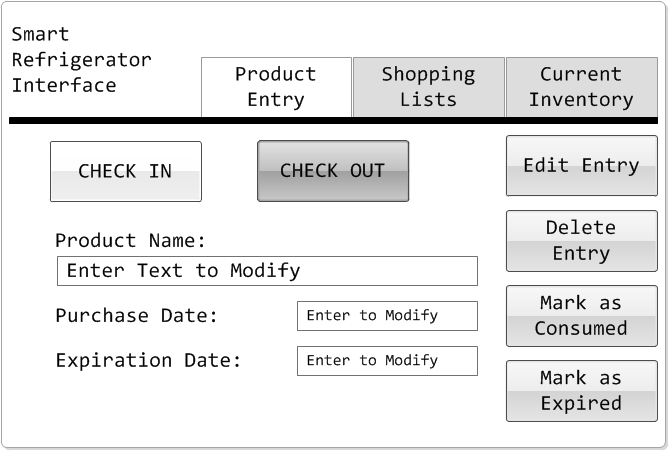
\includegraphics[scale=0.5]{MockUp1}
\caption{Product Entry Tab Layout}
\label{mock1}
\end{center}
\end{figure}

\begin{figure}[h!]
\begin{center}
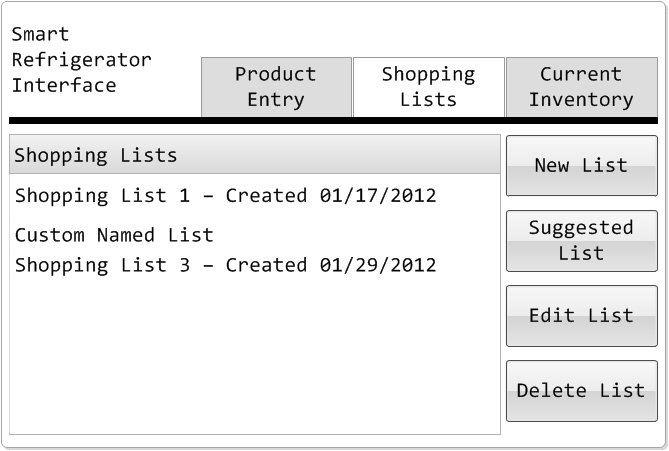
\includegraphics[scale=0.5]{MockUp2}
\caption{Shopping List Tab Layout}
\label{mock2}
\end{center}
\end{figure}
\pagebreak
\begin{figure}[h!]
\vspace{0.5cm}
\begin{center}
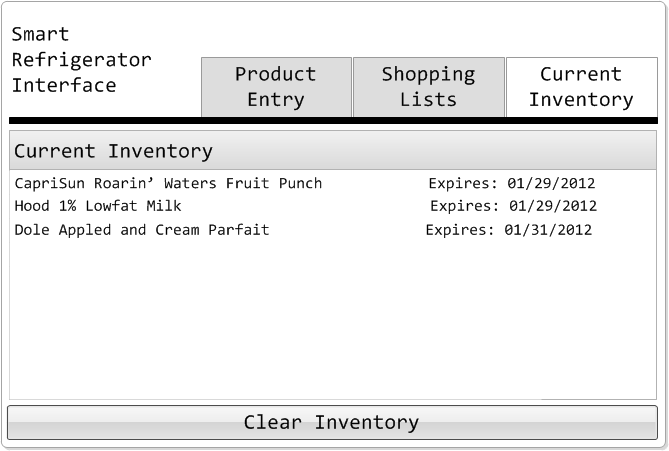
\includegraphics[scale=0.5]{MockUp3}
\caption{Current Inventory Tab Layout}
\label{mock3}
\end{center}
\end{figure}

\begin{figure}[h!]
\begin{center}
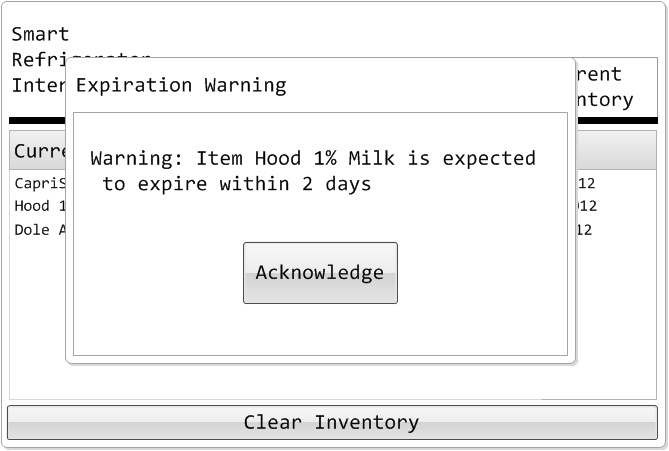
\includegraphics[scale=0.5]{MockUp4}
\caption{Expiration Warning Pop-Up Layout}
\label{mock4}
\end{center}
\end{figure}
\pagebreak
\quad \newline
The mobile interface will be divided into similar tabs, which will limit the amount of data exchanged between the Beagleboard and mobile phone. The mobile application will be updated on a ``need to know" basis only. If additional items have been added to the inventory or new shopping lists have been created, the mobile application will not be notified until the user has opened the application and navigated to the appropriate tab. It is anticipated that the largest data exchanges will need to occur for the shopping lists, since they will require information from multiple items and additional top-level information about the lists. The mobile application will further improve data efficiency by not loading shopping list items until a list has been selected. Navigation to the shopping list tab will generate a query for the top-level information about new or updated shopping lists, but will not delve down into the lists themselves to retrieve item information. Only once a list has been selected will complete updated information about its items be retrieved. This implementation will create additional latency while using the application; faster strategies include a single large update of all data upon launching the application or a background fetch of information while running the application. However, given the high costs of mobile data plans and the lack of widespread WiFi at most grocery stores, limiting the amount of data passed across the network interface is an important consideration for usability.
\newline \quad \newline
The mobile application should also be tolerant of interrupted connections, since telecommunication networks often have spotty coverage. To mitigate the impact of dropped connections, updates should be transferred from the Beagleboard to the mobile application in a sequence of short communications; a large number of small messages will be more robust than a small number of large messages. This structure will facilitate the ``need to know" distribution of information as well. The processes for handling updates to the current inventory and updates to shopping lists are conceptually similar and are illustrated with a common state machine in Figure \ref{fig:state}. Upon launching the application, the update system will enter a waiting state. The update system will remain waiting until a tab is selected or some other action is performed which requires a check for updates, such as expanding a shopping list to view the items within it. The mobile application will  then request the number of relevant updates from the base station software. The state machine will pend until the number of updates is returned and will then enter a state which evaluates whether there are updates remaining. The system will alternate between pending to receive updates and checking whether additional updates are available. The system will return to the waiting state when all the ``need to know" information has been retrieved.
\begin{figure}[h!]
\vspace{0.5cm}
\begin{center}
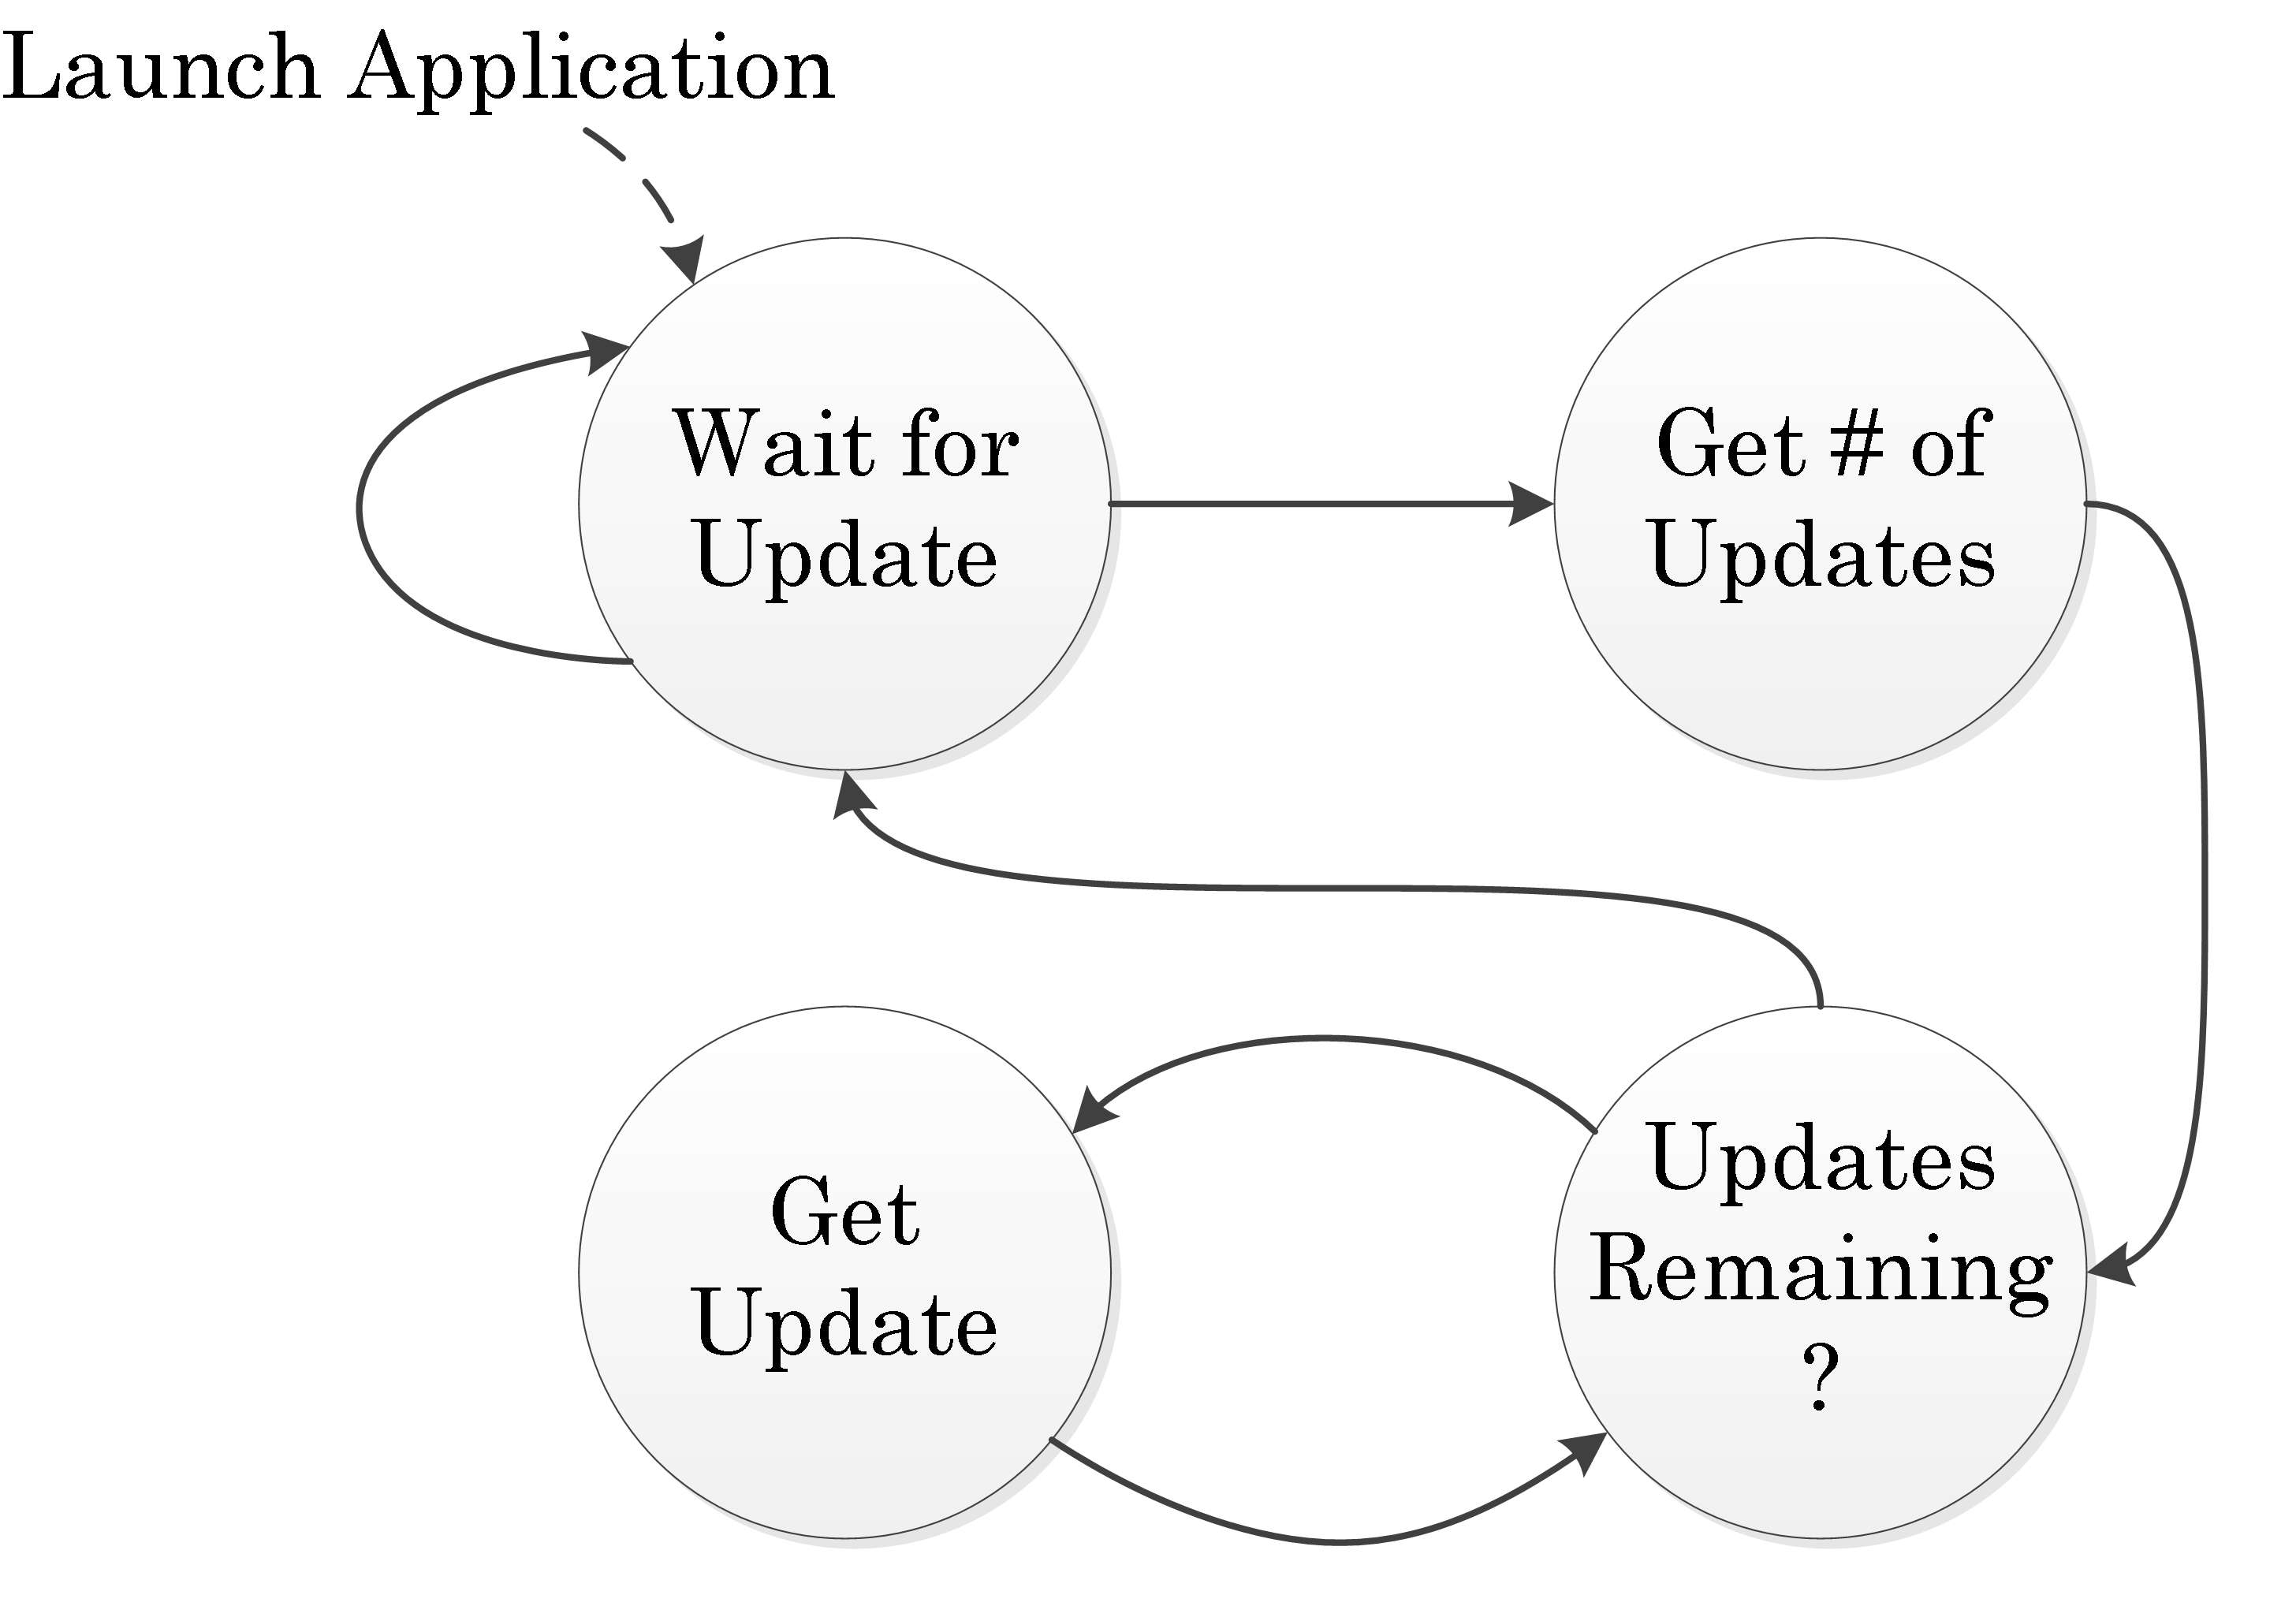
\includegraphics[scale=0.8]{../Graphics/StateMachine}
\caption{State Machine for Database Updates to Mobile Application}
\label{fig:state}
\end{center}
\end{figure}
\newline \quad \newline
The various databases will be implemented as SQL databases on the Beagleboard. SQL databases will certainly be reliable, and testing will be reduced only to ensure correct interaction with the databases. Figure \ref{fig:databases} illustrates the partitioning of data into the multiple databases stored on the Beagleboard. The most intuitive database is the Item Database, which will store the total set of UPC codes and corresponding text descriptions. A quantity field will provide not only the quantity information, but also implicitly provide a check for whether an item is in the current inventory or not. The item database will also store the most recent purchase date for each item. However, only the last purchase date will not be sufficient for the shopping list prediction algorithm, so a separate item history table will be created. The history table will be indexed by UPC and each element will contain a list of purchase dates for that particular item. Also, a shopping list database will be created; in this database each shopping list will be assigned an identification number and name. The shopping lists will also include a flag to indicate whether each shopping list was manually created or generated by the shopping list creation algorithm; the user may find this information useful when evaluating shopping habits. To coordinate between the database of items and the shopping lists themselves, an intermediate linking database will be used to store the actual items included on a shopping list. This database will be indexed by the shopping list identification number and each element will contain a list of item UPC codes.
\begin{figure}[h!]
\begin{center}
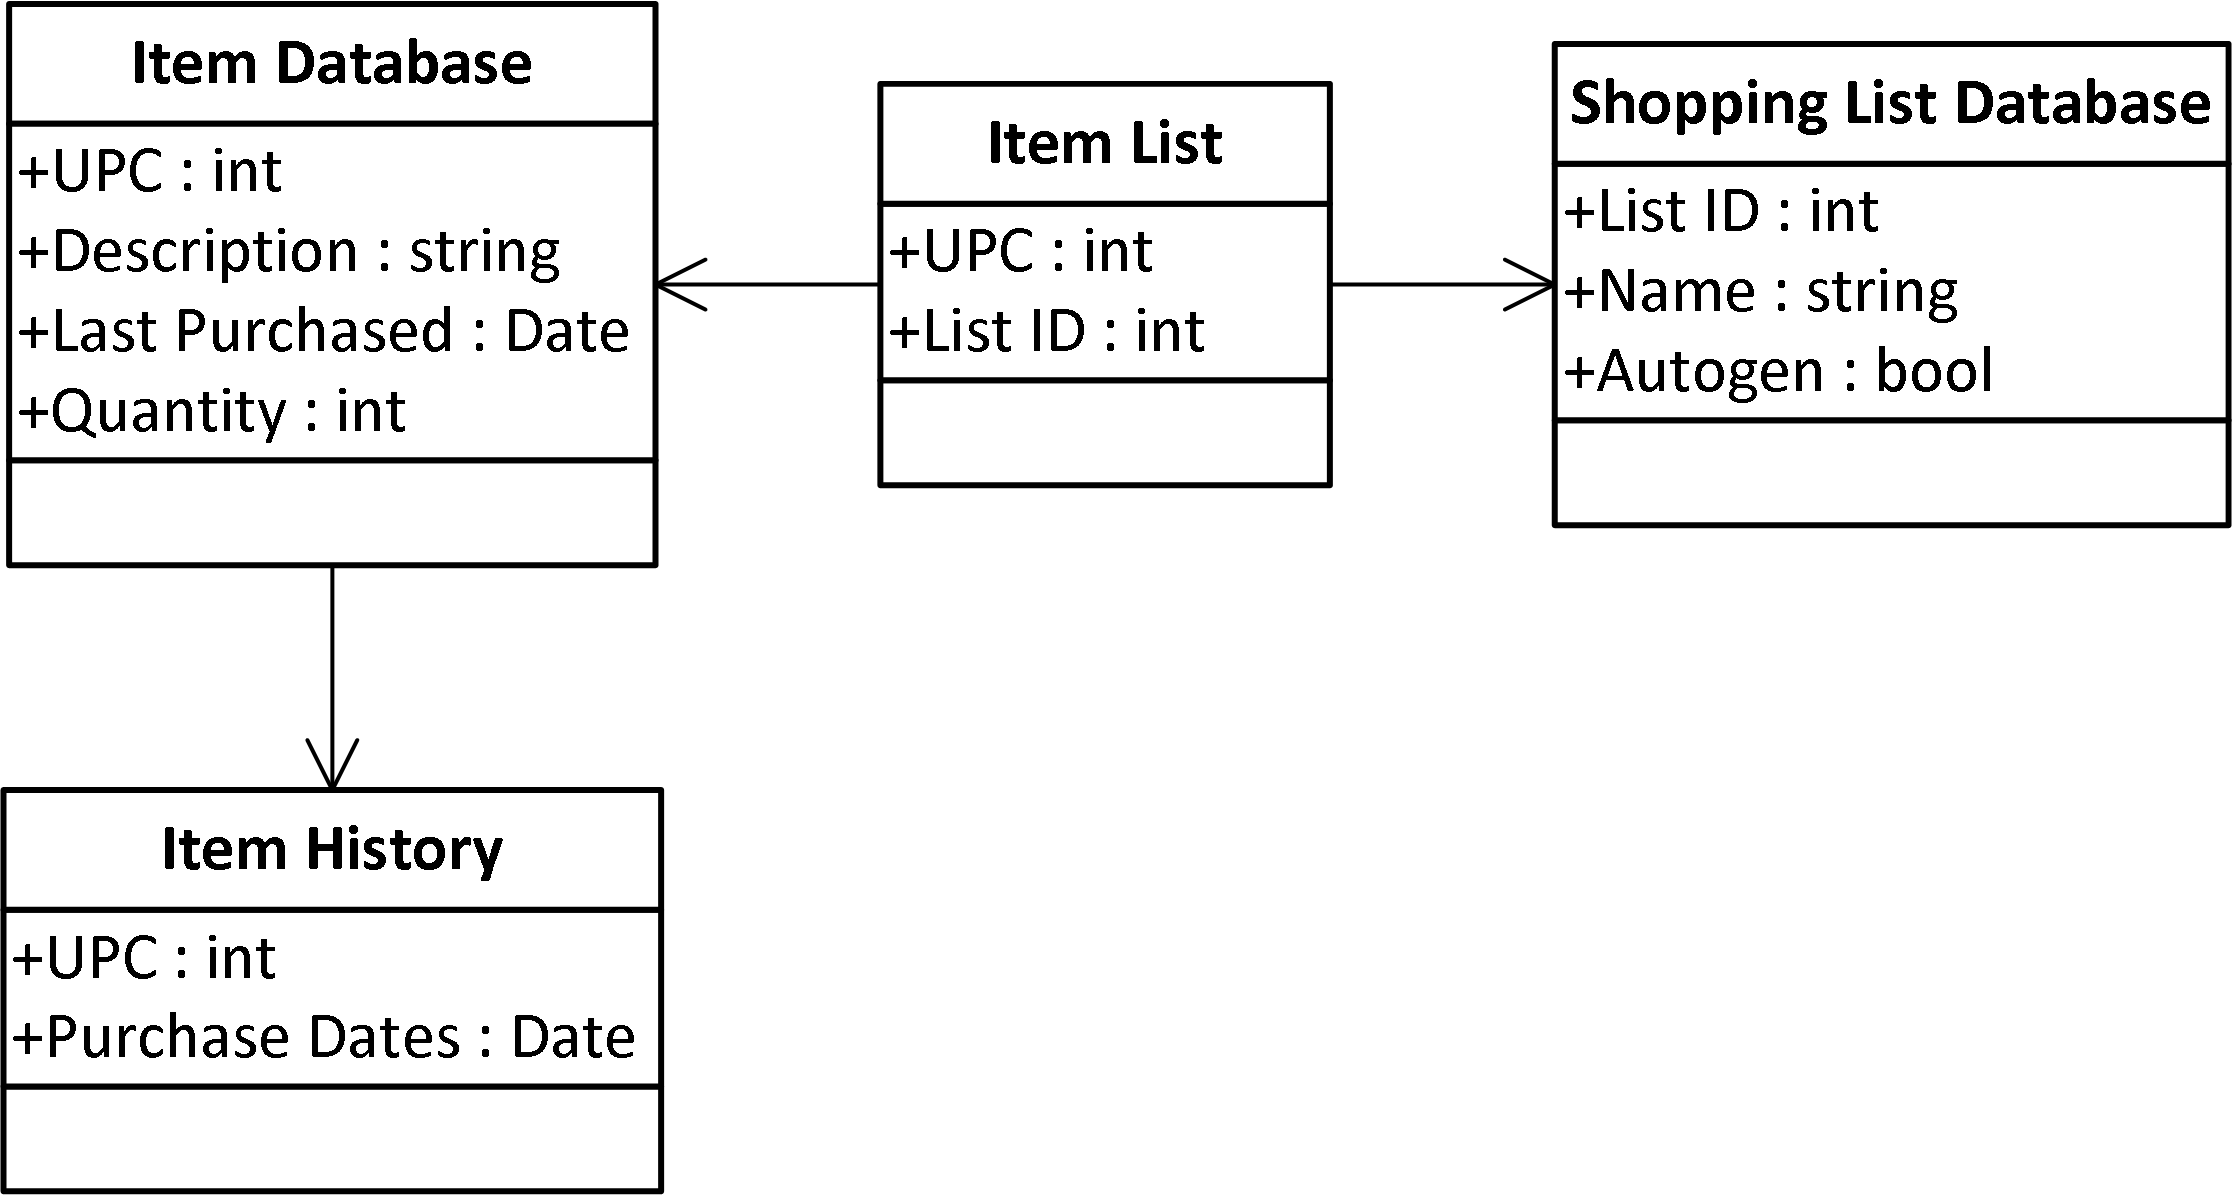
\includegraphics[scale=1.0]{../Graphics/Databases}
\caption{Separation of Information in Databases}
\label{fig:databases}
\end{center}
\end{figure}
\begin{description}
\item[Extensibility] -- The Smart Refrigerator system presented is only a first step toward tackling food waste; integration of the concepts in this prototype into a larger context could provide enormous utility. Possibly the expiration date and purchasing prediction systems could be improved and applied in commercial domains. Both small restaurants and national chains could benefit from more accurate shelf life predictions. The shopping list suggestion algorithm may also be improved by aggregating data from multiple users.
\item[Manufacturability] -- The Smart Refrigerator will be a mainly software system and will therefore be easy to reproduce; the same code package could easily be mass-produced. However, the Beagleboard is a very general processing platform. If this prototype system were manufactured commercially, a more tailored and application specific platform could be desirable. The system does not have a true need for a  complete Linux environment, even though it is ideal for rapid development of a prototype.
\item[Reliability] - The components developed and tested externally, such as the Angstrom operating system, will likely be very robust in comparison with the modules developed specifically for this prototype. The user interfaces and prediction algorithms will be tested extensively, though in both cases it is difficult to fully remove the possibility of error. The mobile interface may not encounter interrupted connections in testing and defects may go unnoticed. The shopping list recommendation algorithm can not be exposed to all shopping habits in testing, and therefore may perform poorly in some untested scenarios. Fortunately, the system will not incur any damage from a failure and will not immediately endanger the user in event of a faliure.
\item[Background] -- Experience with Linux based operating systems throughout the computer science sequence has been helpful. The computer science sequence and software engineering also have provided a valuable introduction to user interface development. The project does not contain significant hardware design, though skills learned in Introduction to Digital Systems may be useful in interfacing with the temperature and humidity sensor.
\item[Multidisciplinary Aspects] -- This prototype system requires coordination between hardware and software and requires a mixture of Computer Engineering and Software Engineering skills. However, multidisciplinary projects often carry a mechanical connotation and this system does not require integration of any mechanical components.
\end{description}
\section{Considerations}
The Smart Refrigerator system proposed is a step toward promoting sustainability and good stewardship of natural resources. Both the New York Times articles mentioned in the statement of needs, and other reports \cite{times, aol}, indicate that approximately 27\% of all food available for consumption is lost to waste. A study published by the UN Food and Agriculture Organization declares the global percentage is even higher, totalling 1.3 billion tons or 33\% overall \cite{dutch}. The system designed will increase awareness about expiring items, with the goal of reducing these figures. Hugh Collins from AOL News speculates that food waste is dismissed subconsciously; many foods are cheap, and the average consumer does not think about the aggregated cost of these small wastes \cite{aol}. By providing reminders to the user, the Smart Refrigerator can remedy this source of waste by keeping the user aware of all their purchases. Expiration of food products themselves is not the only source of waste involved with grocery shopping. Making unnecessarily frequent trips to a store for forgotten or unexpected items also wastes resources. The shopping list recommendations provided by the Smart Refrigerator will hopefully mitigate waste here as well. A final consideration of the system is health and safety, by providing reminders about expiring products the risk of eating expired products will hopefully be decreased. 
\pagebreak
\section{Cost Estimates}
We have submitted a proposal to the ARM student design contest requesting a BeagleBoard-xM and power adapter. If our proposal is accepted we will be able to obtain these parts at no cost. We also already own many of the principle system components; the dorm room refrigerator, android smart phone, and LCD display will not need to be purchased.
\begin{table}[h!]
\vspace{0.5cm}
\begin{center}
\caption{Cost Table}
\label{tab:cost}
\begin{tabular}{| p{2.5in} | p{1.75in} |p{1.75in} |}
\hline
Part & Retail Cost & Our Cost \\
\hline
BeagleBoard-xM & \$149 & \$0 \\
\hline
BeagleBoard-xM Power Adapter & \$14.87 & \$0 \\
\hline
Dorm Room Refrigerator & \$100 & \$0 \\
\hline
Android Smart Phone & \$100 & \$0  \\
\hline
LCD Display & \$80  & \$0 \\
\hline
UPC Barcode Scanner & \$35 & \$35 \\
\hline
USB Keyboard/Keypad & \$10 & \$10 \\
\hline
\hline
\textbf{Total Cost} & \$488.87 & \$45 \\
\hline
\end{tabular}
\end{center}
\end{table}

\section{Testing Strategy}
Testing of the Smart Refrigerator will be divided into unit testing of the various subsystems and then top-level integration testing once the sub-systems have been connected. Some components used within the system, such as the Angstrom operating system and SQL database implementation, which have undergone extensive test prior to use in our system, will only be tested to ensure proper configuration. The principle subsystems tested will be the base station user interface, mobile user interface and network interface, expiration date and shopping list prediction algorithms, and integration with the BeagleBoard.

\subsection{Base Station User Interface Testing}
The main testing focus will be on the user application, both the software running on the base station as well as the web and Android interfaces.  Unit testing will be performed during development of each component, as well as integration testing of the final application. This subsection will focus on top-level testing of the base station user interface as a module, with tests particularly directed at the engineering specifications and user requirements. Tests directly motivated by the requirements specification and engineering specifications are listed below, and a test procedure is tabulated in Table \ref{tab:gui}.
\begin{itemize}
\item The user interface is required to be easy to use and intuitive; in order to verify this someone not involved in the project should contribute to top-level testing of this sub-system. This also can be tested quantitatively; tests should be performed to ensure the most used items are presented on the default tab, and the most frequently used controls are the most accessible.
\item The user interface will provide access to the current inventory, which will be stored using an SQL database. The principle test effort at this step will be verifying integration of the display with the database, not verifying the storage of items themselves.
\item The user interface will provide both read and write access to shopping lists, also stored using an SQL database. Testing of this feature will again focus on the ability of the interface to query and modify database entries, not on the database implementation itself.
\item The user interface must provide a method to update expiration estimates. Testing of this subsystem will not verify that the update is reasonable or correct but simply verify that this user interface action triggers an update from the expiration prediction subsystem.
\item To achieve the principal goal of the system, the user interface must provide a notification of items about to expire. Testing of this subsystem will not verify that the expiration estimate is reasonable or correct, but simply that if triggered by the expiration prediction subsystem the user interface will display an indication.
\end{itemize}

\begin{table}[h!]
\vspace{0.5cm}
\caption{Base Station User Interface Test Cases}
\label{tab:gui}
\begin{tabular}{|c|p{3cm}|p{6cm}|c|c|c|c|c|}
\hline
\multicolumn{8}{|l|}{Test Writer:Steven Strapp} \\
\hline
\hline
\multicolumn{2}{|c|}{Test Case Name:} & \multicolumn{4}{|l|}{Base Station Interface Top-Level Unit Tests}& Test ID \#: & Base-01 \\
\hline
\multicolumn{2}{|c|}{Description:}& \multicolumn{4}{|p{8cm}|}{Verify that the base station user interface meets the requirement and engineering specifications. Some, such as usability will be evaluated qualitatively and are difficult to outline in this way.}&Type:&White Box\\
\hline
\hline
\multicolumn{8}{|l|}{Tester Information}\\
\hline
\multicolumn{2}{|c|}{Name of Tester:}&\multicolumn{4}{|c|}{}&Date: & \\
\hline
\multicolumn{2}{|c|}{Hardware Ver:}&\multicolumn{4}{|c|}{}&Time: & \\
\hline
\hline
\multicolumn{2}{|c|}{Setup:}&\multicolumn{6}{|p{10cm}|}{User interface subsystem should be entirely integrated with prediction subsystems and SQL databases. System should begin without shopping lists or inventory. System date should be made mutable to facilitate quick simulation of expiration.} \\
\hline
\rotatebox{90}{Test \hspace{.2cm}}& Action& \multicolumn{1}{|p{6cm}|}{Expected Result} & \rotatebox{90}{Pass}& \rotatebox{90}{Fail} & \rotatebox{90}{N/A} & \multicolumn{2}{|p{3cm}|}{Comments}\\
\hline
1 & Enter fake \newline product code & Switch to inventory tab,  entered product should be shown. Inventory should be otherwise empty. & & & &\multicolumn{2}{|c|}{}\\
\hline
2 & Wait for fake \newline product to nearly expire & Interface should display a notification indicating expiring item. & & & &\multicolumn{2}{|c|}{}\\
\hline
3 & Use interface to indicate product has not yet \newline expired & Verify that prediction sub-system is triggered to update its expiration estimate for this product. & & & &\multicolumn{2}{|c|}{}\\
\hline
4 & Create fake \newline shopping list & Verify that list becomes accessible through base station and Android interface & & & &\multicolumn{2}{|c|}{}\\
\hline
5 & Modify items on \newline fake shopping list & Verify that changes are retained and visible through base station or Android interface & & & &\multicolumn{2}{|c|}{}\\
\hline
\end{tabular}
\end{table}
\pagebreak
\subsection{Mobile User Interface and Network Interface Testing}
The web and mobile interfaces will have their own set of tests, focused on basic functionality and interoperability on various platforms.  The web interface will be tested on the most popular browsers (Google Chrome, Firefox, and Internet Explorer), as well as some of the most popular mobile platforms (Android, WebOS, and iOS).  The Android interface will need to be tested on various versions of the operating system.  At a minimum, major versions between 2.1 and 4.0 will be tested.  

\begin{table}[h!]
\caption{Mobile App Tests}
\label{tab:mobApp}
\begin{tabular}{|c|p{3cm}|p{6cm}|c|c|c|c|c|}
\hline
\multicolumn{8}{|l|}{Test Writer:Ben Reeves} \\
\hline
\hline
\multicolumn{2}{|c|}{Test Case Name:} & \multicolumn{4}{|p{8cm}|}{Downloading large database updates 
over an \newline intermittent network connection}& Test ID \#: & Mob-01 \\
\hline
\multicolumn{2}{|c|}{Description:}& \multicolumn{4}{|p{8cm}|}{Ensure that the database is correctly downloaded
even if the device's network connection is interrupted. This could be due to 
loss of service, a disabled network adapter, or the device powering down.}&Type:&White Box\\
\hline
\hline
\multicolumn{8}{|l|}{Tester Information}\\
\hline
\multicolumn{2}{|c|}{Name of Tester:}&\multicolumn{4}{|c|}{}&Date: & \\
\hline
\multicolumn{2}{|c|}{Hardware Ver:}&\multicolumn{4}{|c|}{}&Time: & \\
\hline
\hline
\multicolumn{2}{|c|}{Setup:}&\multicolumn{6}{|p{12cm}|}{System should have a fresh 
install of the application and no previous copies of the database downloaded.} \\
\hline
\rotatebox{90}{Step \hspace{.2cm}}& Action& \multicolumn{1}{|p{6cm}|}{Expected 
Result} & \rotatebox{90}{Pass}& \rotatebox{90}{Fail} & \rotatebox{90}{N/A} & 
\multicolumn{2}{|p{3cm}|}{Comments}\\
\hline
1 & Initiate download \newline update of the \newline database & System should connect to the server 
  and begin downloading. & & & &\multicolumn{2}{|c|}{}\\
\hline
2 & Sever device's \newline network \newline connection & System should pause the download upon sensing 
  the interrupted connection. & & & &\multicolumn{2}{|c|}{}\\
\hline
3 & Reconnect device \newline to the network & System should resume download of the database 
  & & & &\multicolumn{2}{|c|}{}\\
\hline
4 & Allow update to \newline complete & System should download the remaining portion of the 
  database& & & &\multicolumn{2}{|c|}{}\\ 
\hline
\end{tabular}
\end{table}
\pagebreak

\begin{table}[h!]
\vspace{0.5cm}
\caption{UI Usability Test}
\label{tab:usability}
\begin{tabular}{|c|p{3cm}|p{6cm}|c|c|c|c|c|}
\hline
\multicolumn{8}{|l|}{Test Writer:Ben Reeves} \\
\hline
\hline
\multicolumn{2}{|c|}{Test Case Name:} & \multicolumn{4}{|l|}{UI Usability Test}& Test ID \#: & UI-01 \\
\hline
\multicolumn{2}{|c|}{Description:}& \multicolumn{4}{|p{8cm}|}{Ensure that the both the web and mobile 
 versions of the User Interface are accessible and intuitive.}&Type:&White Box\\
\hline
\hline
\multicolumn{8}{|l|}{Tester Information}\\
\hline
\multicolumn{2}{|c|}{Name of Tester:}&\multicolumn{4}{|c|}{}&Date: & \\
\hline
\multicolumn{2}{|c|}{Hardware Ver:}&\multicolumn{4}{|c|}{}&Time: & \\
\hline
\hline
\multicolumn{2}{|c|}{Setup:}&\multicolumn{6}{|p{12cm}|}{System should be representative of one which is in
active use; that is, its database should contain both shopping lists and grocery items associated with them.} \\
\hline
\rotatebox{90}{Step \hspace{.2cm}}& Action& \multicolumn{1}{|p{6cm}|}{Expected 
Result} & \rotatebox{90}{Pass}& \rotatebox{90}{Fail} & \rotatebox{90}{N/A} & 
\multicolumn{2}{|p{3cm}|}{Comments}\\
\hline
1 & System is given to a user unfamiliar with its operation and submitted to stress testing & 
  User should experience little difficulty navigating the application and experience no bugs, freezes, or crashes. 
  & & & &\multicolumn{2}{|c|}{}\\
\hline
\end{tabular}
\end{table}
\pagebreak

\begin{table}[h!]
\vspace{0.5cm}
\caption{UI Interoperability Test}
\label{tab:interop}
\begin{tabular}{|c|p{3.5cm}|p{5.5cm}|c|c|c|c|c|}
\hline
\multicolumn{8}{|l|}{Test Writer:Ben Reeves} \\
\hline
\hline
\multicolumn{2}{|c|}{Test Case Name:} & \multicolumn{4}{|l|}{UI Interoperability Test}& Test ID \#: & UI-02 \\
\hline
\multicolumn{2}{|c|}{Description:}& \multicolumn{4}{|p{7.5cm}|}{Ensure that the both the web and mobile \newline
 versions of the User Interface are fully \newline compatible with popular browsers.}&Type:&\multicolumn{1}{|p{1cm}|}{White \newline Box}\\
\hline
\hline
\multicolumn{8}{|l|}{Tester Information}\\
\hline
\multicolumn{2}{|c|}{Name of Tester:}&\multicolumn{4}{|c|}{}&Date: & \\
\hline
\multicolumn{2}{|c|}{Hardware Ver:}&\multicolumn{4}{|c|}{}&Time: & \\
\hline
\hline
\multicolumn{2}{|c|}{Setup:}&\multicolumn{6}{|p{11cm}|}{System should be representative of one which is in
active use; that is, its database should contain both shopping lists and grocery items associated with them.} \\
\hline
\rotatebox{90}{Step \hspace{.2cm}}& Action& \multicolumn{1}{|p{6cm}|}{Expected 
Result} & \rotatebox{90}{Pass}& \rotatebox{90}{Fail} & \rotatebox{90}{N/A} & 
\multicolumn{2}{|p{1cm}|}{Comments}\\
\hline
1 & Interface is accessed via Mozilla Firefox and subjected to stress testing 
  & Interface is displayed properly, no artifacts or misplaced \newline elements apparent.
  & & & &\multicolumn{2}{|c|}{}\\
\hline
2 & Interface is accessed via Google Chrome and subjected to stress testing 
  & Interface is displayed properly, no artifacts or misplaced \newline elements apparent.
  & & & &\multicolumn{2}{|c|}{}\\
\hline
3 & Interface is accessed via Microsoft \newline Internet Explorer \newline and subjected to \newline stress testing 
  & Interface is displayed properly, no artifacts or misplaced \newline elements apparent.
  & & & &\multicolumn{2}{|c|}{}\\
\hline
4 & Interface is accessed via Android 2.1 and subjected to stress \newline testing 
  & Interface is displayed properly, no artifacts or misplaced \newline elements apparent. 
  & & & &\multicolumn{2}{|c|}{}\\
\hline
5 & Interface is accessed via Android 4.0 and subjected to stress \newline testing 
  & Interface is displayed properly, no artifacts or misplaced \newline elements apparent.
  & & & &\multicolumn{2}{|c|}{}\\
\hline
\end{tabular}
\end{table}
\clearpage

\subsection{Shopping List and Expiration Prediction Test}
Testing of the expiration prediction and shopping list prediction subsystems will be difficult if the system's date can not be adjusted artificially; testing should occur over a few minutes rather than a series of days. For expiration date testing, the system's date should be easy to change artificially, so products appear to expire very quickly. The intelligence of the system can then be tested by providing feedback that test products expired more or less quickly than expected, and evaluating the updated predictions. By simply accelerating the rate with which the system changes date, this subsystem can be tested without adding specific test products with low shelf lives and without changing the algorithms to update more frequently. A set of tests is listed for this subsystem below.
\begin{itemize}
\item Enter a product code and verify that the expiration date system is initialized with recommended ``rule of thumb" value.
\item Provide feedback indicating that a product expired before estimate and validate that the estimate is decreased. Also validate the opposite case: providing feedback that a product had not yet expired on estimated date should increase the estimate.
\item Enter a product code and advance the system time until the product is nearly expired. Verify that the prediction subsystem has indicated to controller that the product is nearing expiration.
\item Rescan a product code after regular intervals, indicative of uni-modal shopping habits. Verify that the system recommends the product should be purchased again on this mode. Date may be artificially advanced to facilitate quick testing.
\item Continue from the previous case and add outlier shopping habits. Validate that system continues to recommend purchasing the product again on the mode.
\item Enter various products with different purchasing habits. Verify that the system recommends purchasing the products with the highest probabilities.
\item Rescan a product code after regular intervals, then add significant variation. Observe that system attempts to track  the variation in habits.
\item Rescan a product code after varying intervals, indicative of bi-modal shopping habits. Verify that the system recommends purchasing the product on both modes.
\end{itemize}
\subsection{Integration with BeagleBoard}
Preliminary testing will focus on the BeagleBoard itself and its ability to interact with the desired peripherals.  The system will require an LCD screen, a USB barcode scanner, a network connection, a keypad, and temperature/humidity sensor.  Basic functionality of these components will be tested thoroughly during development, as well as during final system testing. 
\newline \quad \newline
The SQL database used to store all data for the system will be tested once the core of the user application has been coded.  Test scripts will be written to populate the databases with fake data in order to ensure that the database is configured as desired, and to verify that the user application is properly communicating with the database alongside the web interface.
\newline \quad \newline
It is difficult to outline exactly what testing will be required for the processing platform, since it is unclear what compatibility issues will arise that would not be presented by a conventional platform, where ideally the system would be entirely ``plug and play". However, listed below is a baseline sequence of tests.
\begin{itemize}
\item Verify that the BeagleBoard, with power adapter, can power all peripheral devices reliably. No sporadic failures occur, this will be performed as an endurance test.
\item Verify that MAC address of Ethernet interface can be statically assigned and the BeagleBoard can be pinged reliably; this will be performed as an endurance test, cycling power or disconnecting the board multiple times.
\item Verify that the BeagleBoard can reliably interface with the USB scanner and USB keypad, these tests should be performed by writing to a text editor or another program external to the user interface to isolate failures.
\item Verify that the BeagleBoard's consistently receives accurate temperature and humidity measurements from the sensor, via the general purpose input/output pins. The measurements should be verified with an external sensor.
\item Verify that the touchscreen display accurately records users clicks and controls the pointer; tested outside of the user interface to isolate failures.
\item Verify that touchscreen accurately displays the graphical user interface without artifacts or distortion consistently, and ensure all controls on the display are accessible.
\end{itemize}

\section{Risks}
The risks unresolved in the prototype system are best grouped by subsystem. Some unresolved risks are simply due to unknown availability of parts, others require further exploration, and still others are more fundamental risks.
\begin{description}
\item[Availability of LCD Display] -- The ULCD7 Lite is the preferred choice for the display to accompany the Beagleboard. The 7-inch resistive touchscreen is designed to work with the Beagleboard and has drivers built into the Angstrom Linux distribution. However, the touchscreen does not seem to be stocked by online suppliers and our request through the Arm Developer Day proposal process is still pending. Since the Beagleboard provides a DVI-D and S-video output, this risk could be mitigated using a traditional computer monitor if the preferred touch screen is not available. The availability of these alternate interfaces also facilitates development while waiting for the desired part. However, since the base station display is a critical system component, if this risk is not resolved shortly one of the less desirable alternatives will have to be selected.
\item[Mobile Application Data Exchange] -- Exchanging inventory and shopping lists data with the mobile application presents two risk areas: the amount of data plan usage required and interrupted network connections. These risks are partially mitigated by the design, which exchanges data in small increments on a ``need to know" basis only, however the degree to which these risks are truly problematic is not know. For development, the smart phone can be connected with WiFi instead of a costly data connection; however, the data requirements should be tested early on in development to ensure this risk does not become a latent problem. Interrupted connections are considered in the design, but the effectiveness of the design will be difficult to measure since it may be difficult to repeatedly interrupt the data connection.
\item[Practicality of Prediction Algorithms] -- The shopping list prediction algorithm outlined appears optimal for the test data considered. However, the analysis performed did not consider a large sample of shoppers and the conclusions drawn may not be appropriate for a larger population. Also, the prediction algorithm outlined will not perform well with only a few samples; it is unclear how unacceptable this warm-up period will appear to end users. The strategy presented is also quite heavy-handed and may be superfluous for this prototype system. The system will not serve as an effective shopping aid without an accurate prediction system, but a prototype may be acceptable with a much simpler system requiring significantly less effort.
\item[Efficiency of Database Access] -- Efficient practices for database access were not known or considered when partitioning information into separate tables. Efficiency was also not considered when developing the schema for the databases. For example, using the same database to store all possible items and the current inventory may be an inefficient choice. This strategy requires looking over all elements and extracting only those with non-zero quantities. If the system was extended to large commercial applications, or if the Beagleboard was replaced with a more cost-efficient and less powerful alternative, this organization may become a significant risk.
\end{description}
\pagebreak
\section{Milestones}
\begin{table}[h!]
\caption{Table of Milestones}
\begin{center}
\begin{tabular}{| p{6 cm} | p{4.5 cm} | p{4.5 cm}|}
%\begin{tabular}{|l|l|l|}
\hline
\textbf{Milestone} & \textbf{Scheduled Completion\newline Date} & \textbf{Assigned} \\
\hline
BeagleBoard procured & February 10, 2012 & Steven Strapp\\
\hline
Angstrom operating system running on board & February 24, 2012 & Dustin Stroup \\
\hline
Peripherals properly interfacing with board & March 02, 2012 & Dustin Stroup \\
\hline
Basic mobile UI, suitable for debugging & March 9, 2012 & Ben Reeves\\
\hline
Basic base station UI, suitable for debugging & March 9, 2012 & Steven Strapp\\
\hline
Database I/O configured & March 16, 2012 & Ben Reeves \\
\hline
Database and web server hosted by Beagleboard & March 16, 2012 & Dustin Stroup \\
\hline
Testing and integration of temperature and humidity sensor & March 16, 2012 & Steven Strapp \\
\hline
Beagleboard touchscreen display procured & March 16, 2012 & Dustin Stroup \\
\hline
Mobile application integrated with web server & March 30, 2012 & Ben Reeves \\
\hline
User profiling and statistical analysis & March 30, 2012 & Steven Strapp \\
\hline 
Shopping lists, item modification, basic settings & March 30, 2012 & Dustin Stroup \\
\hline
Updated base station UI & April 6, 2012 & Steven Strapp \\
\hline
Updated mobile application & April 6, 2012 & Ben Reeves \\
\hline
Improved robustness of mobile interface& April 13, 2012 & Dustin Stroup \\
\hline
Integration testing and system verification & April 13, 2012 & Ben Reeves \\
\hline
System testing and demo preparation & April 20, 2012 & Steven Strapp \\
\hline
\end{tabular}
\label {MilestoneTable}
\end{center}
\end{table}

\pagebreak

\addcontentsline{toc}{section}{10\hspace{.090in} References}
\begin{thebibliography}{9}
\bibitem{times}
Martin, Andrew. ``One Country's Table Scraps, Another Country's Meal." New York Times. N.p., 18 May 2008. Web. 26 Jan 2012. 
\url{http://www.nytimes.com/2008/05/18/weekinreview/18martin.html?pagewanted=all}.
\bibitem{lg}
Ridden, Paul. ``LG launches first Smart-Grid appliance: the Smart Fridge." gizmag. N.p., 27 Apr 2011. Web. 29 Jan 2012. \url{<http://www.gizmag.com/lg-smart-fridge/18502/>}.
\bibitem{aol}
Collins, Hugh. ``Study: US Food Waste Is a Huge Energy Drain." AolNews. N.p., 02 Oct 2010. Web. 29 Jan 2012. \url{<http://www.aolnews.com/2010/10/02/study-american-food-waste-is-a-huge-energy-drain/>}.
\bibitem{dutch}
Ramaker, Rob. ``Food waste is hard to combat." Resource. N.p., 26 Jan 2012. Web. 29 Jan 2012. \url{<http://resource.wur.nl/en/wetenschap/detail/food_waste_is_hard_to_combat/>}.
 \end{thebibliography}

\end{document}
